%%%% Proceedings format for most of ACM conferences (with the exceptions listed below) and all ICPS volumes.
%%%% As of March 2017, [siggraph] is no longer used. Please use sigconf (above) for SIGGRAPH conferences.
%%%% Proceedings format for SIGPLAN conferences 
% \documentclass[sigplan, anonymous, review]{acmart}
%%%% Proceedings format for SIGCHI conferences
% \documentclass[sigchi, review]{acmart}
%%%% To use the SIGCHI extended abstract template, please visit
% https://www.overleaf.com/read/zzzfqvkmrfzn

%\documentclass[sigplan, anonymous, review]{acmart}
\documentclass[sigconf]{acmart}
%\documentclass[sigconf, anonymous, review]{acmart}
%\documentclass[sigconf]{acmart}


\usepackage{booktabs} % For formal tables
\usepackage{hyperref}
\usepackage{siunitx}
\usepackage{xspace}

\usepackage{listings}
\lstset{   
  breaklines=true,                 % sets automatic line breaking
  captionpos=b,                    % sets the caption-position to bottom
  frame=single,	                   % adds a frame around the code
  xleftmargin=2em,
  framexleftmargin=1.5em,
  keepspaces=true,                 % keeps spaces in text, useful for keeping indentation of code (possibly needs columns=flexible)
  keywordstyle=\color{blue},       % keyword style  
  morekeywords={rule, type, materials, cond, values, conditions, when, then, end},            % if you want to add more keywords to the set
  numbers=left,                    % where to put the line-numbers; possible values are (none, left, right)
  numbersep=5pt,                   % how far the line-numbers are from the code
  numberstyle=\tiny\color{gray}, % the style that is used for the line-numbers  
  rulecolor=\color{black},         % if not set, the frame-color may be changed on line-breaks within not-black text (e.g. comments (green here))
  %showspaces=false,                % show spaces everywhere adding particular underscores; it overrides 'showstringspaces'
  %showstringspaces=false,          % underline spaces within strings only
  %showtabs=false,                  % show tabs within strings adding particular underscores
  %stepnumber=2,                    % the step between two line-numbers. If it's 1, each line will be numbered
  %stringstyle=\color{mymauve},     % string literal style
  %tabsize=2,	                   % sets default tabsize to 2 spaces
  %title=\lstname                   % show the filename of files included with \lstinputlisting; also try caption instead of title
}

%TODO: remover esses pacotes qdo traduzir para ingles
%\usepackage[brazil]{babel}
%\usepackage[utf8]{inputenc}
%\usepackage[T1]{fontenc}


% Copyright
%\setcopyright{none}
%\setcopyright{acmcopyright}
%\setcopyright{acmlicensed}
\setcopyright{rightsretained}
%\setcopyright{usgov}
%\setcopyright{usgovmixed}
%\setcopyright{cagov}
%\setcopyright{cagovmixed}


% DOI
\acmDOI{10.475/123_4}

% ISBN
\acmISBN{123-4567-24-567/08/06}

%Conference
\acmConference[SBCARS 2018]{12th Brazilian Symposium on Software Components, Architectures, and Reuse}{September 2018}{S\~{a}o Carlos, S\~{a}o Paulo, Brazil}
\acmYear{2018}
\copyrightyear{2018}

\acmArticle{4}
\acmPrice{15.00}

%\acmBadgeL[http://ctuning.org/ae/ppopp2016.html]{ae-logo}
%\acmBadgeR[http://ctuning.org/ae/ppopp2016.html]{ae-logo}


\begin{document}

\title[On the Use of Metaprogramming and DSL: An Experience Report]{On the Use of Metaprogramming and Domain Specific Languages: An Experience Report in the Logistics Domain} 


% \author{Pedro Henrique Teixeira Costa, Edna Dias Canedo and Rodrigo Bonif\'{a}acio de Almeida}
% \email{pedro.costa@aluno.unb.br, ednacanedo@unb.br, rbonifacio@unb.br}
% \affiliation{
%  \institution{Computer Science Department, University of Bras\'{i}lia - (UnB)}
%  \streetaddress{P.O. Box 4466}
%  \city{Bras\'{i}lia}
%  \state{DF}
%  \postcode{70910-900}
% }

\renewcommand{\shortauthors}{-}

\newcommand{\callers}{\emph{high-level rules}\xspace}
\newcommand{\shc}{HLR\xspace}

\begin{abstract}
In this paper we present the main design and architectural decisions to build an enterprise system that deals with the distribution of equipment to the Brazilian Army. The requirements of the system are far from trivial, and we have to conciliate the need to extract business rules from the source code (increasing software flexibility) with the requirements of not exposing the use of declarative languages to use a rule-based engine and simplifying the tests of the application. Considering these goals, we present in this paper a seamless integration of meta-programming and domain-specific languages. The use of meta-programming allowed us to isolate and abstract all definitions necessary to externalize the business rules that ensure the correct distribution of the equipment through the Brazilian Army unities. The use of a domain specific language simplified the process of writing automatic test cases related to our domain. Although our architecture targets the specific needs of the Brazilian Army, we believe that logistic systems from other institutions might also benefit from our technical decisions.
\end{abstract}

%
% The code below should be generated by the tool at
% http://dl.acm.org/ccs.cfm
% Please copy and paste the code instead of the example below.
%
\begin{CCSXML}
<ccs2012>
<concept>
<concept_id>10010405.10010406.10010423</concept_id>
<concept_desc>Applied computing~Business rules</concept_desc>
<concept_significance>500</concept_significance>
</concept>
<concept>
<concept_id>10010405.10010476.10010478</concept_id>
<concept_desc>Applied computing~Military</concept_desc>
<concept_significance>500</concept_significance>
</concept>
<concept>
<concept_id>10010147.10010178.10010187</concept_id>
<concept_desc>Computing methodologies~Knowledge representation and reasoning</concept_desc>
<concept_significance>300</concept_significance>
</concept>
<concept>
<concept_id>10011007.10011006.10011041.10011047</concept_id>
<concept_desc>Software and its engineering~Source code generation</concept_desc>
<concept_significance>300</concept_significance>
</concept>
<concept>
<concept_id>10011007.10011006.10011050.10011023</concept_id>
<concept_desc>Software and its engineering~Specialized application languages</concept_desc>
<concept_significance>300</concept_significance>
</concept>
<concept>
<concept>
<concept_id>10011007.10010940.10010971.10010972.10010539</concept_id>
<concept_desc>Software and its engineering~n-tier architectures</concept_desc>
<concept_significance>100</concept_significance>
</concept>
<concept>
<concept_id>10011007.10011074.10011081.10011082.10011083</concept_id>
<concept_desc>Software and its engineering~Agile software development</concept_desc>
<concept_significance>100</concept_significance>
</concept>
</ccs2012>
\end{CCSXML}

\ccsdesc[500]{Applied computing~Business rules}
\ccsdesc[500]{Applied computing~Military}
\ccsdesc[300]{Computing methodologies~Knowledge representation and reasoning}
\ccsdesc[300]{Software and its engineering~Source code generation}
\ccsdesc[300]{Software and its engineering~Specialized application languages}
\ccsdesc[100]{Software and its engineering~n-tier architectures}
\ccsdesc[100]{Software and its engineering~Agile software development}


\keywords{Software Architecture, Generative Programming and Domain Specific Languages, Military Logistics}

%\begin{teaserfigure}
%  \includegraphics[width=\textwidth]{tmp/sampleteaser}
%  \caption{This is a teaser}
%  \label{fig:teaser}
%\end{teaserfigure}


\maketitle

\section{Introduction}\label{sec:Introduction}

% Uma das fases da Logística de Materiais de Emprego Militar das Forças Armadas contempla o planejamento da distribuição de materiais para todas as unidades militares. Essa fase é conhecida como Dotação de Materiais, e envolve a catalogação de materiais, muitas vezes independente de fornecedor, a definição de regras que associam materiais de emprego militar a unidades organizacionais (por exemplo, diretorias, departamentos, batalhões e cargos militares) e a execução das regras para derivar os materiais inicialmente previstos para cada unidade militar e os materiais que devem ser realmente distribuídos para as organizações militares, os quais podem sofrer variações dadas as inclusões e supressões de cargos de uma determinada unidade organizacional do Exército Brasileiro.

One of the logistics' phases to distribute equipments to an army force contemplates the \emph{distribution planning} of materials throughout military units. This phase is known as \emph{material endowment}, and involves several steps, including the specification of 
relevant materials, often independent of vendor; the definition of rules that link military materials and equipments to organizational units (e.g., departments, regiments, and military posts); the execution of the rules for deriving the materials originally intended for each \emph{abstract military unit}; and the designation of the materials that must be actually distributed to the \emph{concrete military organizations}, which may suffer variations due to the inclusions and suppressions of positions for a particular organizational unit of an army force. In the context of this paper, the reader might consider the scenario of the Brazilian Army. 
 
% Sistemas de software de apoio à decisão tornam-se essenciais neste contexto, dada à importância e complexidade dos processos relacionados à Dotação de Materiais de Emprego Militar. Particularmente, as regras usadas para derivar à previsão de material e material previsto não são triviais, e quando implementadas diretamente no código fonte, tornam o sistema difícil de compreender e manter, uma vez que a quantidade de condições que precisam ser expressas é  proporcional à estrutura das unidades organizacionais. Além disso, uma solução "\emph{hard-coding}" não permite aos especialistas do domínio especificarem, de forma trivial, novas regras de derivação. Por essa razão, a externalização das regras de derivação voltadas para a dotação de material é preferencialmente implementada de forma declarativa (e não operacionalmente em uma linguagem de programação como C++ ou Java), usando linguagens, ferramentas ou bibliotecas que suportam algum motor de regras de negócio (\emph{business rule engines}).

Decision support systems are essential in this domain, given the importance and complexity of the processes related to the allocation of military employment materials. In particular, the rules used to predict military materials and equipments are not trivial, and implementing these rules directly in the source code makes the systems difficult to understand and maintain. This problem mostly occurs because the number of conditions that need to be expressed is proportional to complexity of the organizational structure and the number of materials. In the case of an entire army force, this number is noteworthy. In addition, a "\emph{hard-coding}" solution does not allow domain experts to trivially specify and test new derivation rules. For these reasons, it is preferably to implement these rules declaratively, using languages, tools, or libraries that support some sort of inference mechanism.

% Por outro lado, a introdução de linguagens como Prolog~\cite{clocksin2003programming} ou bibliotecas como  Drools~\cite{amador2012}, \cite{bali2009}, \cite{bali2013}, \cite{browne2009} em ambientes corporativos pode sofrer algum tipo de rejeição, particularmente em ambientes cuja arquitetura de sistemas corporativos é bem estabelecida. Além disso, essas soluções requerem uma curva razoável de  aprendizagem, o que pode prejudicar atividades de manutenção de software. 

Nevertheless, introducing either a logic language (e.g, Prolog or Datalog) or a specific library (such as  Drools~\cite{browne2009}) in a complex enterprise system may lead to some type of \emph{architectural 
conflict}, particularly in environments whose whole ecosystem system is well established and based on a set of 
constraints related to both language and libraries usage. Furthermore, these solutions require a reasonable learning curve, which can hamper software maintenance activities.

% Esse artigo descreve as decisões arquiteturais adotadas para implementar o mecanismo de derivação de materiais e materiais previstos para o sistema de dotação de materiais do Exército Brasileiro, que objetiva abstrair completamente o uso de um motor de regras de negócio e permitir que especialistas do domínio simulem a definição e testes de novas regras---usando, na essência, técnicas de programação generativa (como linguagens específicas do domínio e meta-programação). Dessa forma, este artigo apresenta as seguintes contribuições:

This article describes the main design and architectural decisions adopted to implement the mechanisms that assist 
decision makers to plan the distribution of military materials and equipments across the organizational structure 
of the Brazilian Army. These decisions aim to both (a) abstract the adoption of a business rule engine using {\bf metaprogramming} 
and (b) allow domain experts to simulate the definition and testing of rules using 
a {\bf domain specific language}. Accordingly, this paper presents the following contributions:

\begin{itemize}
%   \item O uso de técnicas de programação generativa para o projeto arquitetural e implementação do mecanismo de derivação de materiais e materiais previstos para unidades organizacionais.
\item The use of generative programming techniques for the architectural design and implementation of the derivation mechanism of materials and planned materials for organizational units.

% \item O relato da análise da arquitetura proposta, que reforça que as decisões arquiteturais tomadas foram adequadas e atendem às necessidades dos especialistas do domínio e às restrições técnicas do ambiente corporativo, gerando automaticamente as regras de distribuição de materiais.
\item The analysis report of the proposed architecture, which reinforces that the architectural decisions taken were adequate and attend the needs of the domain specialists and the technical restrictions of the corporate environment, automatically generating the rules of distribution of materials.
\end{itemize} 

% Apesar de discutirmos a distribuição de materiais para o domínio militar (um domínio não trivial), acreditamos que as decisões arquiteturais discutidas nesse artigo possam ser exploradas para outros contextos relacionados à distribuição de materiais e cenários em que se deseja introduzir motores de regras de negócio de forma mais transparente em sistemas corporativos. 

Although we discuss the distribution of materials and equipments for the military domain (which is far from trivial), we believe that the architectural decisions discussed here can be exploited to other logistics and endorsements scenarios in which it is also desirable to transparently introduce the support for rule based engines in enterprise systems.

% Este artigo está organizado como segue. Na Seção \ref{sec:Theory} é apresentado os conceitos relativos a logística de material, arquitetura de software, rule engine e programação generativa que são necessários para o entendimento deste trabalho. A Seção \ref{sec:architecture} apresenta os requisitos arquiteturais e de negócio da solução proposta, bem como os detalhes da implementação. A Seção \ref{sec:case_study} apresenta o estudo de caso desenvolvido para validar a proposta e por fim, a Seção \ref{sec:conclusao} apresenta as conclusões deste trabalho, bem como os trabalhos futuros. 

This article is organized as follows. The Section \ref{sec:logistics} presents the concepts related to material logistics. The Section \ref{sec:rbs} presents the concepts related to business rules and rule based engines. The Section \ref{sec:gp}  presents the concepts related to generative programming that are required for continuous work.  The Section \ref{sec:architecture} presents the architectural decisions and market requirements for the proposed solution, as well as the implementation details. The Section \ref{sec:case_study} presents the case study developed to validate the proposal and finally, the Section \ref{sec:conclusao} presents the conclusions of this work, as well as future work.


%\section{Methodology}\label{sec:Methodology}

%não precisa traduzir essa Seção, não entrara no artigo a ser submetido.

Do ponto de vista da natureza da pesquisa, este trabalho se classifica como uma pesquisa aplicada que tem por objetivo gerar produtos e/ou processos, com finalidades imediatas, com base em conhecimentos prévios. Quanto aos objetivos da pesquisa, caracteriza-se como uma pesquisa exploratória, pois visa proporcionar maior familiaridade com o problema investigado a fim de torná-lo explícito \cite{michel2011metodologia}.

Neste projeto, a coleta e análise dos dados foram realizadas com base em normas, melhores práticas, técnicas, programas, modelos, materiais publicados, constituído principalmente de livros, artigos de periódicos \cite{michel2011metodologia} e materiais disponibilizados pelo Exército Brasileiro para o entendimento de sua Norma de Dotação; caracterizando-se, portanto, como uma pesquisa bibliográfica do ponto de vista do procedimento técnico empregado. Este trabalho também pode ser considerado um estudo de caso, visto que tem objeto de pesquisa restrito, procurando conhecer seus aspectos, suas características ou reconhecer um padrão científico em que o caso possa ser enquadrado, modelado e implementado \cite{travassos2002introduccao}.
\section{Background}
\label{sec:Theory}

% <<TODO: resumir (deixar mais denso), principalmente as "novas" partes: rule engine, generative programming; e colocar as referencias bibliograficas das novas partes>>

\subsection{Logistics}

% A logística é o método usado para implementar estratégia e táticas militares, sendo um método para ganhar vantagem competitiva \cite{rutner2012}. A logística é definida como a arte de mover exércitos, assim como a acomodação e abastecimento dos militares \cite{prebilic2006}. A estratégia e a tática proporcionam o esquema da condução das operações militares, enquanto a logística proporciona os meios. Com isso, logística, estratégica e tática foram, pela primeira vez, posicionadas em um mesmo nível dentro da arte da guerra \cite{marques2014}.

Logistics is the method used to implement military strategy and tactics as a method to gain competitive advantage \cite{rutner2012}. Logistics is defined as the art of moving armies, as well as accommodating and supplying the military \cite{prebilic2006}. Strategy and tactics provide the framework for conducting military operations, while logistics provides the means. Thus, logistic, strategic and tactical were, for the first time, placed on the same level within the art of war \cite{marques2014}.

% Segundo o Ministério da Defesa \cite{brasil2003}, a logística militar é o conjunto de atividades relativas à previsão e à provisão de recursos humanos, materiais e animais, quando aplicável, e dos serviços necessários à execução das missões das forças armadas. A reunião, sob uma única designação, de um conjunto de atividades logísticas afins, correlatas ou de mesma natureza é chamada de função logística. No Brasil, as atividades de logística são agrupadas em sete funções logísticas: Recursos Humanos, Saúde, Suprimento, Manutenção, Transporte, Engenharia e Salvamento. Como o foco deste trabalho é na distribuição de materiais, apenas a função logística suprimento será tratada. A função logística suprimento refere-se ao conjunto de atividades que trata da previsão e provisão do material de todas as classes, necessário às organizações e às forças apoiadas. Tem como atividades o levantamento das necessidades, a obtenção e a distribuição de materiais \cite{brasil2003}.

According to the Ministry of Defense \cite{brasil2003}, military logistics is the set of activities related to the forecasting and provision of human, material and animal resources, when applicable, and the services necessary for the execution of military missions. The meeting, under a single designation, of a set of related logistics activities, related or of the same nature is called the logistic function. In Brazil, logistics activities are grouped into seven logistics functions: Human Resources, Health, Procurement, Maintenance, Transportation, Engineering and Salvage. As the focus of this work is on the distribution of materials, only the logistics supply function will be addressed. The logistics supply function refers to the set of activities that deals with the forecasting and provision of the material of all classes, necessary to the organizations and the forces supported. It has as activities the survey of the necessities, the obtaining and the distribution of materials \cite{brasil2003}.

% Com o objetivo de facilitar a administração e controle dos suprimentos, o Exército Brasileiro utiliza um sistema de catalogação baseado no sistema da North Atlantic Treaty Organization (OTAN) \cite{otan2012} para catalogação, classificando os itens em grupos e classes. A catalogação deve ser realizada de forma a ser obtida a identificação de cada item do material de forma precisa, racional e padronizada, evitando omissão, duplicidade ou dúvidas quanto às características de qualquer material. A catalogação torna-se, então, um instrumento valioso empregado pelos sistemas de gerenciamento logístico ao permitir, no menor tempo possível, a identificação do item de suprimento procurado, sua localização e quantidades disponíveis em estoque \cite{brasil2003}.

In order to facilitate the administration and control of supplies, the Brazilian Army uses a cataloging system based on the North Atlantic Treaty Organization (OTAN) \cite{otan2012} system for cataloging, classifying items into groups and classes. The cataloging must be done in such a way as to obtain the identification of each item of the material in a precise, rational and standardized way, avoiding omission, duplicity or doubts as to the characteristics of any material. Cataloging thus becomes a valuable tool used by logistical management systems by allowing, in the shortest time possible, the identification of the procurement item sought, its location and quantities available in stock \cite{brasil2003}.

% Sistema de suprimento é o conjunto integrado das organizações, pessoal, equipamentos, princípios e normas técnicas destinado a proporcionar o adequado fluxo do suprimento \cite{brasil2003}. A organização e o funcionamento do sistema pressupõem \cite{brasil2003}: 

Supply system is the integrated set of organizations, personnel, equipment, principles and technical standards intended to provide the adequate flow of supply \cite{brasil2003}. The organization and operation of the system presuppose \cite{brasil2003}:

\begin{itemize}
% \item Planejamento e supervisão de todas as ações relacionadas com o suprimento;
\item Planning and supervision of all actions related to the supply;
% \item Normas de solicitação e fornecimento que proporcionem presteza, a fim de atender com oportunidade as necessidades;
\item Request and delivery standards that provide promptness in order to meet needs with opportunity;
% \item Controle capaz de proporcionar todas as informações pertinentes à situação dos estoques e à comparação das necessidades com a disponibilidade;
\item Control able to provide all the information pertinent to the inventory situation and the comparison of the needs with the availability;
% \item Órgãos executivos, nos diversos escalões de comando, encarregados da obtenção e da distribuição;
\item Executive Bodies, at the various levels of command, responsible for procurement and distribution;
% \item Pessoal e instalações para receber, armazenar e distribuir os diversos itens;
\item Personnel and facilities to receive, store and distribute the several items;
% \item Utilização do menor número possível de instalações intermediárias, buscando minimizar o manuseio de itens.
\item Use of as few intermediate facilities as possible, seeking to minimize the handling of items.
\end{itemize}

% Os níveis de estoque previstos no sistema são mantidos por um sistema de suprimento automático. Para tanto, são utilizados instrumentos de cálculo como quadros de dotação de material,  fatores de consumo, suprimento e reposição, tabelas, dentre outros. Quando surgem necessidades especiais de reajustamento, são realizados pedidos para a adequação da distribuição de suprimentos \cite{brasil2003}.

The inventory levels foreseen in the system are maintained by an automatic supply system. For this, calculation instruments are used, such as tables of material endowment, consumption factors, supply and replacement, tables, among others. When special adjustment needs arise, requests are made for the adequacy of the distribution of supplies \cite{brasil2003}.

\subsection{Software Architecture}

% Arquitetura de software se tornou mais ampla e complexa devido às características dos sistema atuais, tais como: distribuídos e interconectados, escaláveis horizontalmente e prontos para um ambiente de computação em nuvem, publicados automaticamente em ambientes diversos, atualizáveis com mínimo de downtime, resilientes e adaptativos \cite{hohpe2016}. Há também uma diferença em relação à abordagem tradicional, que trata a arquitetura como um conjunto de componentes e conectores, ao tratar a arquitetura como um conjunto de decisões arquiteturais realizadas no sistema \cite{bosch2004}, \cite{jansen2005}.

Software architecture has become more extensive and complex due to the characteristics of the current systems, such as: distributed and interconnected, scalable horizontally and ready for a cloud computing environment, automatically published in diverse, updatable environments with minimal downtime, resilient and adaptive \cite{hohpe2016}. There is also a difference from the traditional approach, which treats architecture as a set of components and connectors, by treating architecture as a set of architectural decisions made in the system \cite{bosch2004}, \cite{jansen2005}.

% Arquitetura de software é um conjunto de estruturas necessárias para raciocinar sobre um sistema, que compreendem elementos de software, relações entre eles e propriedades de ambos \cite{bass2013software}. Existem três categorias de estruturas arquiteturais \cite{clements2011documenting}, \cite{bass2013software}. A arquitetura de software está relacionada diretamente aos atributos de qualidade do sistema; permite raciocinar sobre o impacto de mudanças enquanto o sistema evolui; a documentação da arquitetura melhora a comunicação entre os interessados e serve como base de treinamento de novos membros da equipe; serve como uma receita para a implementação do sistema; ajuda no planejamento de custos e cronograma de atividades; possibilita o reuso de soluções \cite{bass2013software}. 

Software architecture is a set of structures necessary to reason about a system, which comprise elements of software, relations between them and properties of both \cite{bass2013software}. There are three categories of architectural structures \cite{clements2011documenting}, \cite{bass2013software}. The software architecture is directly related to the quality attributes of the system; it allows to reason about the impact of changes as the system evolves; architecture documentation improves communication among stakeholders and serves as a training base for new team members; serves as a recipe for the implementation of the system; help with cost planning and schedule of activities; enables the reuse of solutions \cite{bass2013software}.

% Os atributos de qualidade considerados relevantes para a arquitetura proposta neste trabalho são: 

The quality attributes considered relevant for the architecture proposed in this work are:

\begin{itemize}

% \item Simplicidade na definição das regras de distribuição de materiais, transformando definições de alto nível  em definições baseadas em regras de motor de inferência, o que facilita a manutenção e extrai tais definições do código fonte de uma aplicação. Isso motivou o uso de programação generativa (em termos de meta programação) e um motor de inferência específico para a linguagem Java;

\item Simplicity in defining material distribution rules by transforming high-level definitions into definitions based on inference engine rules, which facilitates maintenance and extracts such definitions from the source code of an application. This motivated the use of generative programming (in terms of meta programming) and an inference engine specific to the Java language;

% \item Facilidade para execução de testes automatizados, motivando a definição de uma Domain-Specific Languages (DSL) para descrever conceitos relacionados à dotação de materiais para o Exército Brasileiro. A partir DSL, são gerados casos de testes baseados em "especificações executáveis" e classes que instanciam objetos do domínio. 

\item Ease of execution of automated tests, motivating the definition of a Domain-Specific Languages (DSL) to describe concepts related to the endowment of materials for the Brazilian Army. From DSL, test cases are generated based on "executable specifications" and classes that instantiate objects of the domain.

\end{itemize}


\subsection{Rule Engine}

% Uma regra de negócio é uma declaração compacta, atômica e bem formada sobre um aspecto do negócio que pode ser expresso em termos que podem estar diretamente relacionados com o negócio e seus colaboradores, usando linguagem simples e não ambígua que é acessível a todas as partes interessadas: proprietário da empresa, analista de negócios, arquitetos, técnicos, cliente, dentre outros \cite{graham2007}. Esse tipo de estrutura é muito importante para as organizações, já que elas precisam lidar cada vez mais com  cenários complexos. Estes cenários são compostos por um grande número de decisões individuais, que trabalham em conjunto para fornecer uma avaliação complexa da organização como um todo \cite{salatino2016}.

A business rule is a compact, atomic, and well-formed statement about an aspect of the business that can be expressed in terms that may be directly related to the business and its employees using simple and unambiguous language that is accessible to all stakeholders: business owner, business analyst, architects, technicians, client, among others \cite{graham2007}. This type of structure is very important for organizations, as they need to deal more and more with complex scenarios. These scenarios consist of a large number of individual decisions, working together to provide a complex assessment of the organization as a whole \cite{salatino2016}.

% Sistemas baseados em regras (Rule Based Systems -- RBS), também conhecidos como production systems ou expert systems, são a forma mais simples de inteligência artificial, usando regras como representação do conhecimento \cite{grosan2011}. Ao invés de representar o conhecimento de forma declarativa e estática como um conjunto de coisas que são verdadeiras, RBS representa o conhecimento em termos de um conjunto de regras que diz o que fazer ou o que concluir em diferentes situações \cite{grosan2011}. Essas regras são também conhecidas como: condição-ação, produções, situação-ação ou se-então \cite{russell2010}.

Rule Based Systems (RBS), also known as production systems or expert systems, are the simplest form of artificial intelligence, using rules such as knowledge representation \cite{grosan2011}. Instead of representing knowledge in a declarative and static way as a set of things that are true, RBS represents knowledge in terms of a set of rules that tells what to do or what to accomplish in different situations \cite{grosan2011}. These rules are also known as: condition-action, productions, situation-action, or if-then \cite{russell2010}.

% Expert Systems são sistemas que são capazes de oferecer soluções para problemas específicos em um determinado domínio ou que são capazes de dar conselhos, tanto de um modo quanto em um nível comparável ao de especialistas na área \cite{lucas1991}. Os especialistas tendem a expressar a maioria de suas técnicas de solução de problemas em termos de um conjunto de regras situação-ação, e isto sugere que sistemas baseados em regras deve ser o método de escolha para a construção de tais sistemas \cite{hayesRoth1985}. O apelo intuitivo das regras para resolver problemas mal estruturados resulta em regras que, muitas vezes, são fáceis para os não-programadores lerem e escreverem \cite{grossner1993}. Alguns problemas podem ser facilmente solucionados usando linguagens de programação tradicionais, enquanto escrever um sistema baseado em regras é a maneira mais fácil de resolver os outros problemas \cite{friedman2003}, dando um importante impulso ao desenvolvimento de sistemas especialistas similares em outras áreas de conhecimento \cite{lucas1991}.

Expert Systems are systems that are capable of providing solutions to specific problems in a given domain or that are capable of giving advice, both in a way and at a level comparable to that of \cite{lucas1991} area experts. Experts tend to express most of their problem-solving techniques in terms of a set of situation-action rules, and this suggests that rule-based systems should be the method of choice for building such systems \cite{hayesRoth1985}. The intuitive appeal of rules to solve poorly structured problems results in rules that are often easy for non-programmers to read and write \cite{grossner1993}. Some problems can be easily solved using traditional programming languages, while writing a rules-based system is the easiest way to solve the other problems \cite{friedman2003}, giving an important impetus to the development of similar expert systems in other areas of knowledge \cite{lucas1991}.

% Todo RBS consiste de elementos básicos: uma \textbf{knowledge base} - KB) para armazenar o conhecimento, e o \textbf{inference engine}, também conhecido como rule engine, que possui algoritmos para manipular o conhecimento representado na base de conhecimento \cite{grosan2011}, \cite{lucas1991}, \cite{gallacher1989}, \cite{hayesRoth1985}, \cite{buchanan1983}, \cite{abraham2005}. A base de conhecimento armazena fatos e regras \cite{hayesRoth1985}. Fato é uma afirmação usualmente estática sobre propriedades, relações ou proposições \cite{hayesRoth1985} e deve ser algo relevante para o estado inicial do sistema \cite{grosan2011}. Uma regra é uma declaração condicional que vincula determinadas condições a ações ou resultados \cite{abraham2005}, podendo expressar políticas, preferências e restrições \cite{gilman2015}. As regras podem ser usadas para expressar o conhecimento dedutivo, como relacionamentos lógicos e, assim, suportar tarefas de inferência, verificação ou avaliação \cite{hayesRoth1985}.

All RBS consists of basic elements: a \textbf{knowledge base} (KB) to store knowledge, and inference engine, also known as rule engine, which has algorithms to manipulate the knowledge represented in the knowledge base \cite{grosan2011}, \cite{lucas1991}, \cite{gallacher1989}, \cite{hayesRoth1985}, \cite{buchanan1983}, \cite{abraham2005}. The knowledge base stores facts and rules \cite{hayesRoth1985}. Fact is an usually static statement about properties, relations, or propositions \cite{hayesRoth1985} and should be something relevant to the initial state of the system \cite{grosan2011}. A rule is a conditional statement that links certain conditions to actions or results \cite{abraham2005}, being able to express policies, preferences, and constraints \cite{gilman2015}. Rules can be used to express deductive knowledge, such as logical relationships, and thus support inference, verification, or evaluation tasks \cite{hayesRoth1985}.

% Uma regra se-então assume a forma "se x é A então y é B". A parte condicional (SE) é conhecida como: antecedente, premissa, condição ou left-hand-side (LHS). A outra parte é conhecida como: consequente, conclusão, ação ou right-hand-side (RHS) \cite{grosan2011}, \cite{abraham2005}. Existem alguns algoritmos que são utilizados em sistemas baseados em regras, como: LEAPS \cite{batory1994}, TREAT \cite{wang1992}, \cite{miranker1991}, PHREAK \cite{salatino2016}, além de variações do Rete \cite{forgy1982}, como: Rete-OO \cite{sottara2010}, \cite{salatino2016}, Rete-ADH \cite{kim2014} e Rete-ECA \cite{lee2014}.

A rule if-then takes the form "if x is A then y is B". The conditional part (SE) is known as: antecedent, premise, condition or left-hand-side (LHS). The other part is known as: consequent, conclusion, action or right-hand-side (RHS) \cite{grosan2011}, \cite{abraham2005}. There are some algorithms that are used in rule-based systems, such as: LEAPS \cite{batory1994}, TREAT \cite{wang1992}, \cite{miranker1991}, PHREAK \cite{salatino2016}, besides variations of the Rete \cite{forgy1982}, such as: Rete-OO \cite{sottara2010}, \cite{salatino2016}, Rete-ADH \cite{kim2014} and Rete-ECA \cite{lee2014}.

% O sistema baseado em regras funciona da seguinte maneira \cite{grosan2011}: começa com uma base de conhecimento, que contém todo o conhecimento apropriado codificado em regras se-então, e uma memória de trabalho, que pode ou não conter inicialmente quaisquer dados, asserções ou informações inicialmente conhecidas. O sistema examina todas as condições da regra (LHS) e determina um subconjunto, o conjunto de conflitos, das regras cujas condições são satisfeitas com base na memória de trabalho. Deste conjunto de conflitos, uma dessas regras é acionada. A escolha da regra é baseada em uma estratégia de resolução de conflitos. Quando a regra é acionada, quaisquer ações especificadas em sua cláusula THEN (RHS) são executadas. Essas ações podem modificar a memória de trabalho, a própria base de regras ou fazer praticamente qualquer outra coisa que o programador do sistema decida incluir. Esse loop de regras de disparo e ações de execução continua até que um critério de finalização seja atendido. Esse critério de término pode ser dado pelo fato de que não há mais regras cujas condições são satisfeitas ou uma regra é disparada cuja ação especifica que o programa deve ser finalizado.

The rules-based system works as follows \cite{grosan2011}: it starts with a knowledge base, which contains all appropriate knowledge coded in if-then rules, and a working memory, which may or may not initially contain any data, assertions or information initially known. The system examines all rule conditions (LHS) and determines a subset, the set of conflicts, of rules whose conditions are satisfied based on working memory. From this set of conflicts, one of these rules is triggered. The choice of rule is based on a conflict resolution strategy. When the rule is triggered, any actions specified in its THEN clause (RHS) are executed. These actions can modify the working memory, the rule base itself, or do almost anything else that the system programmer chooses to include. This trigger rules loop and execute actions continue until a termination criterion is met. This end criterion can be given by the fact that there are no more rules whose conditions are satisfied or a rule is triggered whose action specifies that the program should be finalized.

% O Drools é uma plataforma de integração de lógica de negócios (BLiP - Business Logic integration Platform), escrito na linguagem Java. É um projeto de código aberto que é apoiado pelo JBoss e Red Hat, Inc\cite{bali2009}. É licenciado sob a Licença Apache, Versão 2.0 \cite{browne2009}. Atualmente encontra-se na versão 7.7.0. Neste trabalho foi usado o módulo Drools Expert, usado para executar as regras, juntamente com o algoritmo PHREAK. Este algoritmo foi introduzido na versão 6 do Drools para abordar alguns dos principais problemas do Rete, incorporando todo o código existente de ReteOO e todos os seus aprimoramentos, além de ter sido inspirado em outros algoritmos, como: LEAPS, Rete/UL \cite{doorenbos1995} e Collection-Oriented Match \cite{acharya1993}. Apesar de ser uma evolução do algoritmo Rete, não é mais classificado como uma implementação Rete \cite{drools2017}.

Drools is a business logic integration platform (BLiP) written in the Java language. It is an open source project that is supported by JBoss and Red Hat, Inc \cite{bali2009}. It is licensed under the Apache License, Version 2.0 \cite{browne2009}. Currently it is in version 7.7.0. In this work it is used the Drools Expert module, used to execute the rules, along with the PHREAK algorithm. This algorithm was introduced in version 6 of Drools to address some of Rete's main problems, incorporating all existing ReteOO's code and all its enhancements, as well as being inspired by other algorithms, such as: LEAPS, Rete/UL \cite{doorenbos1995} and Collection-Oriented Match \cite{acharya1993}. Although it is an evolution of the Rete algorithm, it is no longer classified as a Rete implementation \cite{drools2017}.

\subsection{Generative Programming}

% A maioria das tecnologias orientadas a objeto focam no desenvolvimento de sistemas únicos ao invés de famílias de sistemas. Portanto, elas não suportam adequadamente a reutilização de software, devido há algumas deficiências \cite{czarnecki1999}.  Design patterns e frameworks representam uma contribuição extremamente valiosa da tecnologia orientada a objeto para a reutilização de software \cite{gamma1994}. Frameworks de software são uma tecnologia de reuso de software que promove a reutilização de arquiteturas inteiras dentro de um domínio de aplicativo estritamente definido \cite{cechticky2003}. No entanto, elas ainda precisam ser acompanhadas por uma abordagem sistemática de engenharia para e com reuso \cite{czarnecki1999}.

Most object-oriented technologies focus on developing single systems rather than system families. Therefore, they do not adequately support software reuse, due to some weaknesses \cite{czarnecki1999}. Design patterns and frameworks represent an extremely valuable contribution of object-oriented technology to software reuse \cite{gamma1994}. Software frameworks are a software reuse technology that promotes the reuse of entire architectures within a strictly defined application domain \cite{cechticky2003}. However, they still need to be accompanied by a systematic engineering approach to and with reuse \cite{czarnecki1999}.

% Generative Programming (GP) está relacionada ao projeto e implementação de componentes de software que podem ser combinados para gerar sistemas especializados e altamente otimizados, cumprindo requisitos específicos \cite{czarnecki1998}. Com esta abordagem, em vez de desenvolver as soluções a partir do zero, soluções específicas de domínio são geradas a partir de componentes de software reutilizáveis \cite{arora2009}. GP é aplicada sobre a fabricação de produtos de software a partir de componentes em um sistema de forma automatizada (e dentro de restrições econômicas), ou seja, a forma como outras indústrias têm produzido bens mecânicos, eletrônicos e outros por décadas \cite{barth2002}.

Generative Programming (GP) is related to the design and implementation of software components that can be combined to generate specialized and highly optimized systems, fulfilling specific requirements \cite{czarnecki1998}. With this approach, instead of developing solutions from scratch, domain-specific solutions are generated from reusable software components \cite{arora2009}. GP is applied on the manufacturing of software products from components in a system in an automated way (and within economic constraints), i.e., how other industries have been producing mechanical, electronic and other goods for decades \cite{barth2002}.

% A ideia principal na GP é semelhante àquela que levou as pessoas a mudar de linguagens Assembly para linguagens de alto nível. Isto é, elevando o nível de abstração com o qual um programador ou designer deve lidar e automatizar todas as traduções das abstrações de alto nível para os componentes de implementação. O nível de abstração é um dos atributos mais importantes de uma linguagem de programação \cite{paska2009}. Se a linguagem abstrair dos detalhes da implementação, o código pode ser mais facilmente entendido e verificado. Em técnicas GP, os programadores definem um modelo do sistema que apenas define o conteúdo dos dados e a lógica dos aplicativos. Então, programas semelhantes aos compiladores traduzem esses modelos para os programas ou códigos de máquina reais automaticamente. A partir dos compiladores tradicionais, pode haver vários compiladores de modelos que traduzem um único modelo para várias plataformas, dependendo das necessidades de diferentes usuários \cite{azimi2003}.

The main idea in GP is similar to the one that led people to switch from Assembly languages to high-level languages. That is, raising the level of abstraction with which a programmer or designer must handle and automate all translations of high-level abstractions to the implementation components. The level of abstraction is one of the most important attributes of a programming language \cite{paska2009}. If the language abstracts from the implementation details, the code can be more easily understood and verified. In GP techniques, programmers define a system model that only defines data content and application logic. Then, compiler-like programs translate these templates to the actual programs or machine codes automatically. From the traditional compilers, there may be several compilers of models that translate a single model to multiple platforms, depending on the needs of different users \cite{azimi2003}.

% De acordo com Barth et al \cite{barth2002}, programação generativa é definida como um paradigma de desenvolvimento de software baseado na modelagem de famílias de sistemas de software que, dada uma especificação de requisitos, um intermediário ou produto final altamente customizado e otimizado pode ser automaticamente fabricado sob demanda a partir de implementação elementar e reutilizável. Os objetivos da GP são \cite{czarnecki1998}: diminuir a lacuna conceitual entre o código do programa e os conceitos de domínio; alcançar alta capacidade de reutilização e adaptabilidade; simplificar o gerenciamento de muitas variantes de um componente; e aumentar eficiência (tanto no espaço quanto no tempo de execução). Existem diversas técnicas de programação generativa e outros paradigmas com objetivos similares, tais como: Generic Programming, Domain-Specific Languages (DSLs), e Aspect-Oriented Programming (AOP) \cite{czarnecki1998}.

According to Barth et al \cite{barth2002}, generative programming is defined as a paradigm of software development based on modeling families of software systems that, given a specification of requirements, a highly customized and optimized intermediate or end product can be automatically fabricated on demand from elementary and reusable implementation. The objectives of GP are \cite{czarnecki1998}: to reduce the conceptual gap between program code and domain concepts; achieve high reusability and adaptability; simplify the management of many variants of a component; and increase efficiency (both in space and at run time). There are several generative programming techniques and other paradigms with similar objectives, such as: Generic Programming, Domain-Specific Languages (DSLs), and Aspect-Oriented Programming (AOP) \cite{czarnecki1998}.

\subsubsection{Template Engine}

% Conceitos independentes devem ser representados de forma independente e devem ser combinados apenas quando necessário. Quando esse princípio é violado, conceitos não relacionados são agrupados ou dependências desnecessárias são criadas. De qualquer forma, obtém-se um conjunto de componentes menos flexível a partir do qual os sistemas são compostos. Os templates fornecem uma maneira simples de representar uma ampla variedade de conceitos gerais e formas simples de combiná-los \cite{stroustrup1997}.

Independent concepts should be represented independently and should be combined only when necessary. When this principle is violated, unrelated concepts are grouped or unnecessary dependencies are created. Either way, a less flexible set of components is obtained from which the systems are composed. Templates provide a simple way to represent a wide variety of general concepts and simple ways to combine them \cite{stroustrup1997}.

% De acordo com He and Zheng \cite{he2009}, template engine é uma ferramenta genérica para gerar uma saída textual a partir de arquivos de templates e dados. Podem ser usados no desenvolvimento de software que necessita da geração automática de código conforme propósitos específicos \cite{benato2017}. A necessidade de páginas da web geradas dinamicamente levou ao desenvolvimento de inúmeros templates engine na tentativa de tornar o desenvolvimento de aplicações web mais fácil, melhorar a  flexibilidade, reduzir os custos de manutenção, e permitir codificação em paralelo e desenvolvimento em Linguagem HTML. Estes atraentes benefícios, que têm impulsionado a proliferação de templates engine, derivam inteiramente de um único princípio: separar a especificação da lógica de negócio e do cálculo de dados de uma página, de como uma página exibe tais informações. Com especificações encapsuladas de forma separada, template engine promovem  reutilização de componentes, aparências plugáveis de sites, pontos únicos de mudança para componentes e alta clareza geral do sistema \cite{parr2004}.  

According to He and Zheng \cite{he2009}, template engine is a generic tool for generating textual output from template and data files. They can be used in the development of software that requires the automatic generation of code according to specific purposes \cite{benato2017}. The need for dynamically generated web pages has led to the development of numerous engine templates in an effort to make web application development easier, improve flexibility, reduce maintenance costs, and enable parallel encoding and development in HTML language. These attractive benefits, which have boosted the proliferation of templates engine, derive entirely from a single principle: separate the specification of business logic and calculation of data from a page, from how a page displays such information. With separately encapsulated specifications, template engine promotes reuse of components, pluggable website appearances, single points of change for components, and high overall system clarity \cite{parr2004}.

% Além de serem muito utilizados na geração dinâmica de páginas web, os templates são usados em outras tarefas, tais como: geração de classes Java \cite{arnoldus2007}, arquivos de configuração \cite{costa2015}, arquivos contendo comandos SQL, entre outros. Um template é um documento de texto que combina marcadores de posição (placeholders) e fórmulas linguísticas usadas para descrever algo em um domínio específico \cite{arnoldus2007}, \cite{segura2017}. Os templates facilitam a comunicação entre os profissionais, contribuindo para a disseminação da pesquisa e fornecem um guia útil para iniciantes\cite{segura2017}.

In addition to being widely used in dynamic web page generation, templates are used in other tasks such as: generation of Java \cite{arnoldus2007} classes, configuration files \cite{costa2015}, files containing SQL commands, among others. A template is a text document that combines placeholders and linguistic formulas used to describe something in a specific domain \cite{arnoldus2007}, \cite{segura2017}. Templates facilitate communication among professionals, contribute to the dissemination of research, and provide a useful guide for beginners \cite{segura2017}.

% O processo de geração de código baseado em templates utiliza, como entrada, templates e um conjunto de modelos (dados). A linguagem na qual o template é escrito é conhecida como metalinguagem \cite{arnoldus2011}. O template engine age como um avaliador para gerar código, podendo ser visto como um metaprograma pois manipula código \cite{arnoldus2011}. O modelo é um artefato que descreve o domínio da aplicação em um alto nível de abstração, em uma linguagem de programação ou de modelagem. O modelo é usado pelo avaliador para substituir os marcadores de posição em um template. Esses espaços reservados contêm expressões para obter dados do modelo \cite{arnoldus2007}.

The process of generation of code based on templates uses, as input, templates and a set of models (data). The language in which the template is written is known as metalanguage \cite{arnoldus2011}. The template engine acts as an evaluator to generate code, and can be seen as a metaprogram because it handles code \cite{arnoldus2011}. The model is an artifact that describes the domain of the application in a high level of abstraction, in a programming language or modeling. The template is used by the evaluator to replace placeholders in a template. These placeholders contain expressions to get data from the model \cite{arnoldus2007}.

% Existem vários tipos de template engine: Tapestry, WebMacro, Velocity, PTG, UniT, Tea, WebObjects, FreeMarker, ColdFusion, Template Toolkit, Mason, Thymeleaf, e Pebble \cite{parr2004}. Neste trabalho foi utilizado o template engine Freemarker, que é um software open-source projetado para gerar texto a partir de templates \cite{radjenovic2009}. O Freemarker pode ser considerado o substituto do Apache Velocity e encontra-se na incubadora de projetos da Apache Software Foundation (ASF), que apoia o seu desenvolvimento e é amplamente usado nos projetos da família Apache, como o NetBeans \cite{wengner2016}.

There are several types of template engine: Tapestry, WebMacro, Velocity, PTG, UniT, Tea, WebObjects, FreeMarker, ColdFusion, Template Toolkit, Mason, Thymeleaf, and Pebble \cite{parr2004}. In this work we used the Freemarker template engine, which is an open-source software designed to generate text from templates \cite{radjenovic2009}. Freemarker can be considered the substitute for Apache Velocity and is in the Apache Software Foundation (ASF) project incubator, which supports its development and is widely used in Apache family projects such as NetBeans \cite{wengner2016}. 

% O Freemarker foi escolhido por apresentar as seguintes vantagens: é um software de código aberto; é um modelo de propósito geral; é mais rápido que outros; fornece facilidades de uso (por exemplo, suporte JavaScript Object Notation (JSON), variáveis compartilhadas, carregadores de modelos, entre outros); possui suporte automatizado em Java IDE (Integrated Development Environment); seus templates não são compilados para classes, ou seja, um template pode ser carregado ou recarregado durante o tempo de execução sem reimplementar o aplicativo; e formata automaticamente valores numéricos, datas e horas de acordo com a localização (\textit{locale}) \cite{benato2017}, \cite{parr2006}.

Freemarker was chosen because it has the following advantages: it is open source software; it is a general purpose model; is faster than others; provides ease of use (for example, JavaScript Object Notation (JSON) support, shared variables, model loaders, and so on); has automated support in Java IDE (Integrated Development Environment); their templates are not compiled for classes, that is, a template can be loaded or reloaded at runtime without reimplementing the application; and automatically formats numeric values, dates and times according to location (\textit{locale}) \cite{benato2017}, \cite{parr2006}.

\subsubsection{Domain Specific Language}

% Uma linguagem é um conjunto de sentenças válidas, servindo como mecanismo para expressar intenções \cite{parr2010}, \cite{bentley1987}.  A criação de uma nova linguagem é uma tarefa demorada, requer experiência, sendo geralmente realizada por engenheiros especializados em linguagens \cite{karsai2014}. Para implementar uma linguagem, deve-se construir uma aplicação que leia sentenças e reaja apropriadamente às frases e símbolos de entrada que descobre \cite{parr2013}. 

A language is a set of valid sentences, serving as a mechanism for expressing intentions \cite{parr2010}, \cite{bentley1987}. Creating a new language is a time-consuming task, requires experience, and is usually performed by engineers specializing in languages \cite{karsai2014}. To implement a language, one must construct an application that reads sentences and reacts appropriately to the phrases and input symbols it discovers \cite{parr2013}.

% A necessidade de novas linguagens para vários domínios em crescimento está aumentando, assim como o surgimento de ferramentas mais sofisticadas que permitem aos engenheiros de software definir um novo idioma com um esforço razoável. Como resultado, um número crescente de DSLs estão sendo desenvolvidas para aumentar a produtividade dos desenvolvedores dentro de domínios específicos \cite{karsai2014}. Com sua forte relação com as técnicas de engenharia dirigidas por modelos, elas agora estão recebendo mais atenção com o uso em diferentes áreas relacionadas ao software, sendo orientadas a negócios ou técnicas \cite{collet2014}.

The need for new languages for many growing domains is increasing, as well as the emergence of more sophisticated tools that allow software engineers to define a new language with reasonable effort. As a result, a growing number of DSLs are being developed to increase developer productivity within specific domains \cite{karsai2014}. With their strong relationship with model-driven engineering techniques, they are now receiving more attention with use in different areas related to the software, being business or technical oriented \cite{collet2014}.

% Domain Specific Languages (DSL) são idiomas de especificação ou linguagens de programação com alto nível de abstração, simples e concisas \cite{raja2010}, focadas em domínios específicos, sendo projetadas para facilitar a construção de aplicativos, usualmente de forma declarativa, com expressividade limitada e linhas reduzidas de código, que resolvem esses problemas específicos \cite{neeraj2017}. Uma DSL é uma linguagem de programação de computadores de expressividade limitada, por meio de notações e abstrações apropriadas, focada e geralmente restrita a um domínio de problema específico \cite{fowler2013}, \cite{vanDeursen2000}. DSLs têm o potencial de reduzir a complexidade do desenvolvimento de software, aumentando o nível de abstração para um domínio. De acordo com o domínio da aplicação, diferentes notações (textual, gráfica, tabular) são usadas \cite{pfeiffer2008}.

Domain Specific Languages (DSL) are specification languages or programming languages with high level of abstraction, simple and concise \cite{raja2010}, focused on specific domains, and are designed to facilitate the construction of applications, usually declaratively, with limited expressiveness lines of code, which solve these specific problems \cite{neeraj2017}. A DSL is a computer language of limited expressiveness, through appropriate notations and abstractions, focused and generally restricted to a specific problem domain \cite{fowler2013}, \cite{vanDeursen2000}. DSLs have the potential to reduce the complexity of software development by increasing the level of abstraction for a domain. According to the application domain, different notations (textual, graphical, tabular) are used \cite{pfeiffer2008}.

% Programação orientada a linguagem é um estilo geral de desenvolvimento que opera sobre a ideia de construir software em torno de um conjunto de linguagens específicas de domínio \cite{fowler2005}. Várias áreas do sistema são identificadas e uma DSL é criada para cada uma dessas áreas identificadas \cite{fowler2008}.

Language-oriented programming is a general style of development that operates on the idea of building software around a set of domain-specific languages \cite{fowler2005}. Several areas of the system are identified and a DSL is created for each of these identified areas \cite{fowler2008}.

% Language workbench é um termo para descrever uma nova classe de ferramentas de desenvolvimento de software, projetadas para construir software através de um ambiente rico de múltiplas e integradas DSLs \cite{fowler2008}. Essas ferramentas apoiam a definição, reutilização e composição eficientes de linguagens e suas IDEs (Integrated Development Environment), tornando acessível o desenvolvimento de novas linguagens e apoiando a programação orientada a linguagem, na qual conjuntos de linguagens sintática e semanticamente integradas podem ser construídos com um esforço comparativamente pequeno \cite{erdweg2013}. Uma característica de uma language workbench é a capacidade de editar a representação abstrata de um programa, em oposição à maneira convencional de manipular arquivos de texto para modificar um programa \cite{schmitt2014}.

Language workbench is a term to describe a new class of software development tools, designed to build software through a rich environment of multiple and integrated DSLs \cite{fowler2008}. These tools support the efficient definition, reuse and composition of languages and their Integrated Development Environment (IDEs), making the development of new languages accessible and supporting language-oriented programming, in which syntactically and semantically integrated sets of languages can be constructed with a comparatively small effort \cite{erdweg2013}. A feature of a language workbench is the ability to edit the abstract representation of a program, as opposed to the conventional way of manipulating text files to modify a program \cite{schmitt2014}.

% O uso das linguagens workbenches está crescendo, bem como o número e variedade das próprias workbenches. Uma desvantagem desse crescente número de sistemas é que a terminologia usada e os recursos suportados por diferentes workbenches são tão diferentes que tanto os usuários quanto os desenvolvedores devem se esforçar para entender os princípios comuns e as decisões de projeto \cite{erdweg2015}. Alguns exemplos de language workbenches \cite{schmitt2014}, \cite{erdweg2013}: JastAdd, Rascal, Spoofax, Xtext, Jetbrains MPS e Intentional. Conforme definido por Bettini \cite{bettini2016}, Xtext é um framework do Eclipse \cite{gallardo2003}, \cite{kulkarni2015} para implementar GPLs e DSLs. Permite implementar linguagens rapidamente e, acima de tudo, abrange todos os aspectos de uma infraestrutura de linguagem completa, a partir do parser, gerador de código ou intérprete, até uma integração completa do Eclipse IDE com todos os recursos típicos.

The use of workbenches languages is growing, as well as the number and variety of the workbenches themselves. A disadvantage of this growing number of systems is that the terminology used and the features supported by different workbenches are so different that users and developers alike must strive to understand common principles and design decisions \cite{erdweg2015}. Some examples of language workbenches \cite{schmitt2014}, \cite{erdweg2013}: JastAdd, Rascal, Spoofax, Xtext, Jetbrains MPS and Intentional. As defined by Bettini \cite{bettini2016}, Xtext is an Eclipse framework \cite{gallardo2003}, \cite{kulkarni2015} to implement GPLs and DSLs. Lets you implement languages quickly and, above all, covers all aspects of a complete language infrastructure, from the parser, code generator or interpreter, to a full integration of the Eclipse IDE with all the typical features.

% Para iniciar uma implementação DSL, o Xtext só precisa de uma especificação gramatical semelhante à ANTLR. A partir dessa gramática são gerados o lexer, parser, o modelo AST (Abstract Syntax Tree), a construção do AST para representar o programa analisado e o editor do Eclipse com todos os recursos do IDE. Todas as preocupações do próprio Xtext e do código gerado pelo Xtext podem ser customizadas via injeção de dependência \cite{prasanna2009}. Para as mais preocupantes, o comportamento padrão do Xtext geralmente é bom. Para as preocupações que precisam de customização (validação, vinculação/escopo, entre outros), o Xtext fornece uma API fácil de usar. O Xtext utiliza intensamente o EMF (Eclipse Modeling Framework) \cite{blewitt2013}. A AST criada pelo parser do Xtext é um modelo EMF. O modelo Ecore correspondente pode ser derivado automaticamente da gramática ou ser especificado explicitamente. Assim, o Xtext permite fácil integração com ferramentas do ecossistema Eclipse Modeling, como as linguagens de transformação Model-to-Model ou Model-to-Text. Outro exemplo é integrar o Xtext com ferramentas gráficas como o GMF (Graphical Modeling Framework) \cite{eysholdt2010}.

To start a DSL implementation, Xtext only needs a grammatical specification similar to ANTLR. From this grammar are generated the lexer, parser, AST (Abstract Syntax Tree) model, the construction of AST to represent the analyzed program and the Eclipse editor with all IDE resources. All the concerns of Xtext itself and the code generated by Xtext can be customized via dependency injection \cite{prasanna2009}. For the most worrying, the standard behavior of Xtext is generally good. For concerns that need customization (validation, linking/scope, among others), Xtext provides an easy-to-use API. Xtext strongly uses the EMF (Eclipse Modeling Framework) \cite{blewitt2013}. The AST created by the Xtext parser is an EMF model. The corresponding Ecore template can be automatically derived from grammar or explicitly specified. Thus, Xtext allows easy integration with Eclipse Modeling ecosystem tools, such as Model-to-Model or Model-to-Text transformation languages. Another example is to integrate Xtext with graphical tools such as the GMF (Graphical Modeling Framework) \cite{eysholdt2010}.

% Neste trabalho foi usado o Xtext para implementação de uma DSL, visando a declaração de regras de distribuição de materiais para facilitar a criação de testes manuais e automáticos. 

In this work Xtext was used to implement a DSL, aiming the declaration of material distribution rules to facilitate the creation of manual and automatic tests.

%\section{Requisitos Arquiteturais do SISDOT}\label{sec:requirements}

Este trabalho propõe uma solução arquitetural para a modernização do Sistema de Dotação de Material de Emprego Militar (SISDOT) do Exército Brasileiro. O SISDOT é responsável por manter todos os materiais utilizados pelo Exército Brasileiro (EB), como por exemplo: cantil, fuzil, metralhadora, combustível, viaturas, dentre outros. Estes materiais na maioria das vezes são de uso individual ou coletivo, e em alguns casos essenciais para o exercício das atividades de uma Organização Militar (OM). A estrutura de cada OM é detalhada por um documento que detalha os cargos que preenchem sua estrutura organizacional, o Quadro de Cargos (QC) \cite{brasil2015}.

O SISDOT além de manter o tipo, classe e família dos materiais, é responsável por gerar uma lista de todos os materiais de emprego militar que serão distribuídos nas Organizações Militares do Exército Brasileiro, de acordo com os seus cargos. Essa lista é denominada de "Chamador". O Chamador é utilizado para que possa ser efetuado o Quadro de Dotação de Material (QDM). O QDM por sua vez é usado para a geração do Quadro de Dotação de Material Previsto (QDMP). 

O Quadro de Dotação de Material (QDM) é o documento, baseado no QC, que prevê a quantidade de MEM necessária ao cumprimento das atividades estabelecidas na base doutrinária da OM operativa \cite{brasil2015}. O QDM é de fundamental importância para as atividades do EB uma vez que o mesmo determina as Normas de Dotação (ND) dos materiais de emprego militar, ou seja, uma norma de dotação classifica o cargo do militar e o material que o mesmo necessita para executar o seu trabalho, seja esse material de uso individual ou de uso coletivo. Além disso, um material também pode ser de uso essencial para o exercício da atividade militar.

\textbf{As Normas de Dotação} (ND) são regras que orientam o estabelecimento da distribuição dos diversos materiais militares (denominados Itens Genéricos --IG) por cargos e frações de uma organização militar. Quando a ND é padronizada, ou seja, tem um alcance generalizado para um Cargo e ou uma Fração, a ND deve descrever essa propriedade/intenção. Por exemplo, IG (10201009 -- Equipamento de Uso Individual Completo) -- ND = 1, significa que será distribuído 1 por militar em uma OM do tipo Operacional. Neste caso, verifica-se que o alcance dessa ND atinge a todos os militares das Organizações Militares Operacionais.

A modernização do SISDOT compreende novas funcionalidades, bem como melhorias em funcionalidades existentes no sistema atual. As principais funcionalidades do SISDOT são:

\begin{itemize}

\item Cadastrar Tipo de Material;
Cadastrar Classe de Material;
Cadastrar Família de Material;
Cadastrar Material de Emprego Militar;
Gerar Chamador -- Editar, Clonar e Excluir;
Gerar QDM -- Editar, Clonar, Validar, Revogar ou Excluir;
Gerar QDMP --  Editar, Clonar, Validar, Revogar ou Excluir;
Cadastrar Norma de Dotação Provisória
Gerar Norma de Dotação a partir do Chamador;
Cadastrar Siglas;
Cadastrar Observação;
Cadastrar Síntese;
Gerar Relatórios -- Materiais, Chamador, Norma de Distribuição, QDM e QDMP.
\end{itemize}


\section{Architectural Decisions}
\label{sec:architecture} 

SISDOT is based on the client-server architectural style (according to 
a typical Java enterprise application), where the components interact to each other by requesting 
services from other components~\cite{clements2011documenting}. 
SISDOT is also organized into logical groups of 
components (known as tiers)---a strategy often used in the 
client-server architectural style. The multi-tier architectural pattern 
can be classified as a \emph{component and connector} pattern, 
depending on the criterion used to define the tiers~\cite{bass2013software}. 
Indeed, there are several criteria, such as component type, sharing of the execution environment, 
and so on~\cite{clements2011documenting}.

The multi-tier pattern also induces some topological constraints 
that govern how the components might interact with other components. 
Specifically, connectors might only exist 
between components of the same tier or that reside in an adjacent 
tier~\cite{clements2011documenting}. In addition, according to Bass et al., 
the organization of a system using tiers supports software maintenance, facilitates the definition of 
security policies, and might increase the performance, availability, and modifiability of 
the systems~\cite{bass2013software}. 


\subsection{Runtime Architectural Description for QDM Generation}

In order to further detail and illustrate the SISDOT architecture, 
and the main architectural decisions to address the constraints introduced 
in Section~\ref{sec:logistics}, here we present a scenario that refers to the 
generation of QDMs using a runtime architectural 
description, whose components, relationships, and interactions are illustrated
in Figure~\ref{fig:fig:runtime_qdm}). 

%\begin{figure*}
\begin{figure}[!ht] \centering
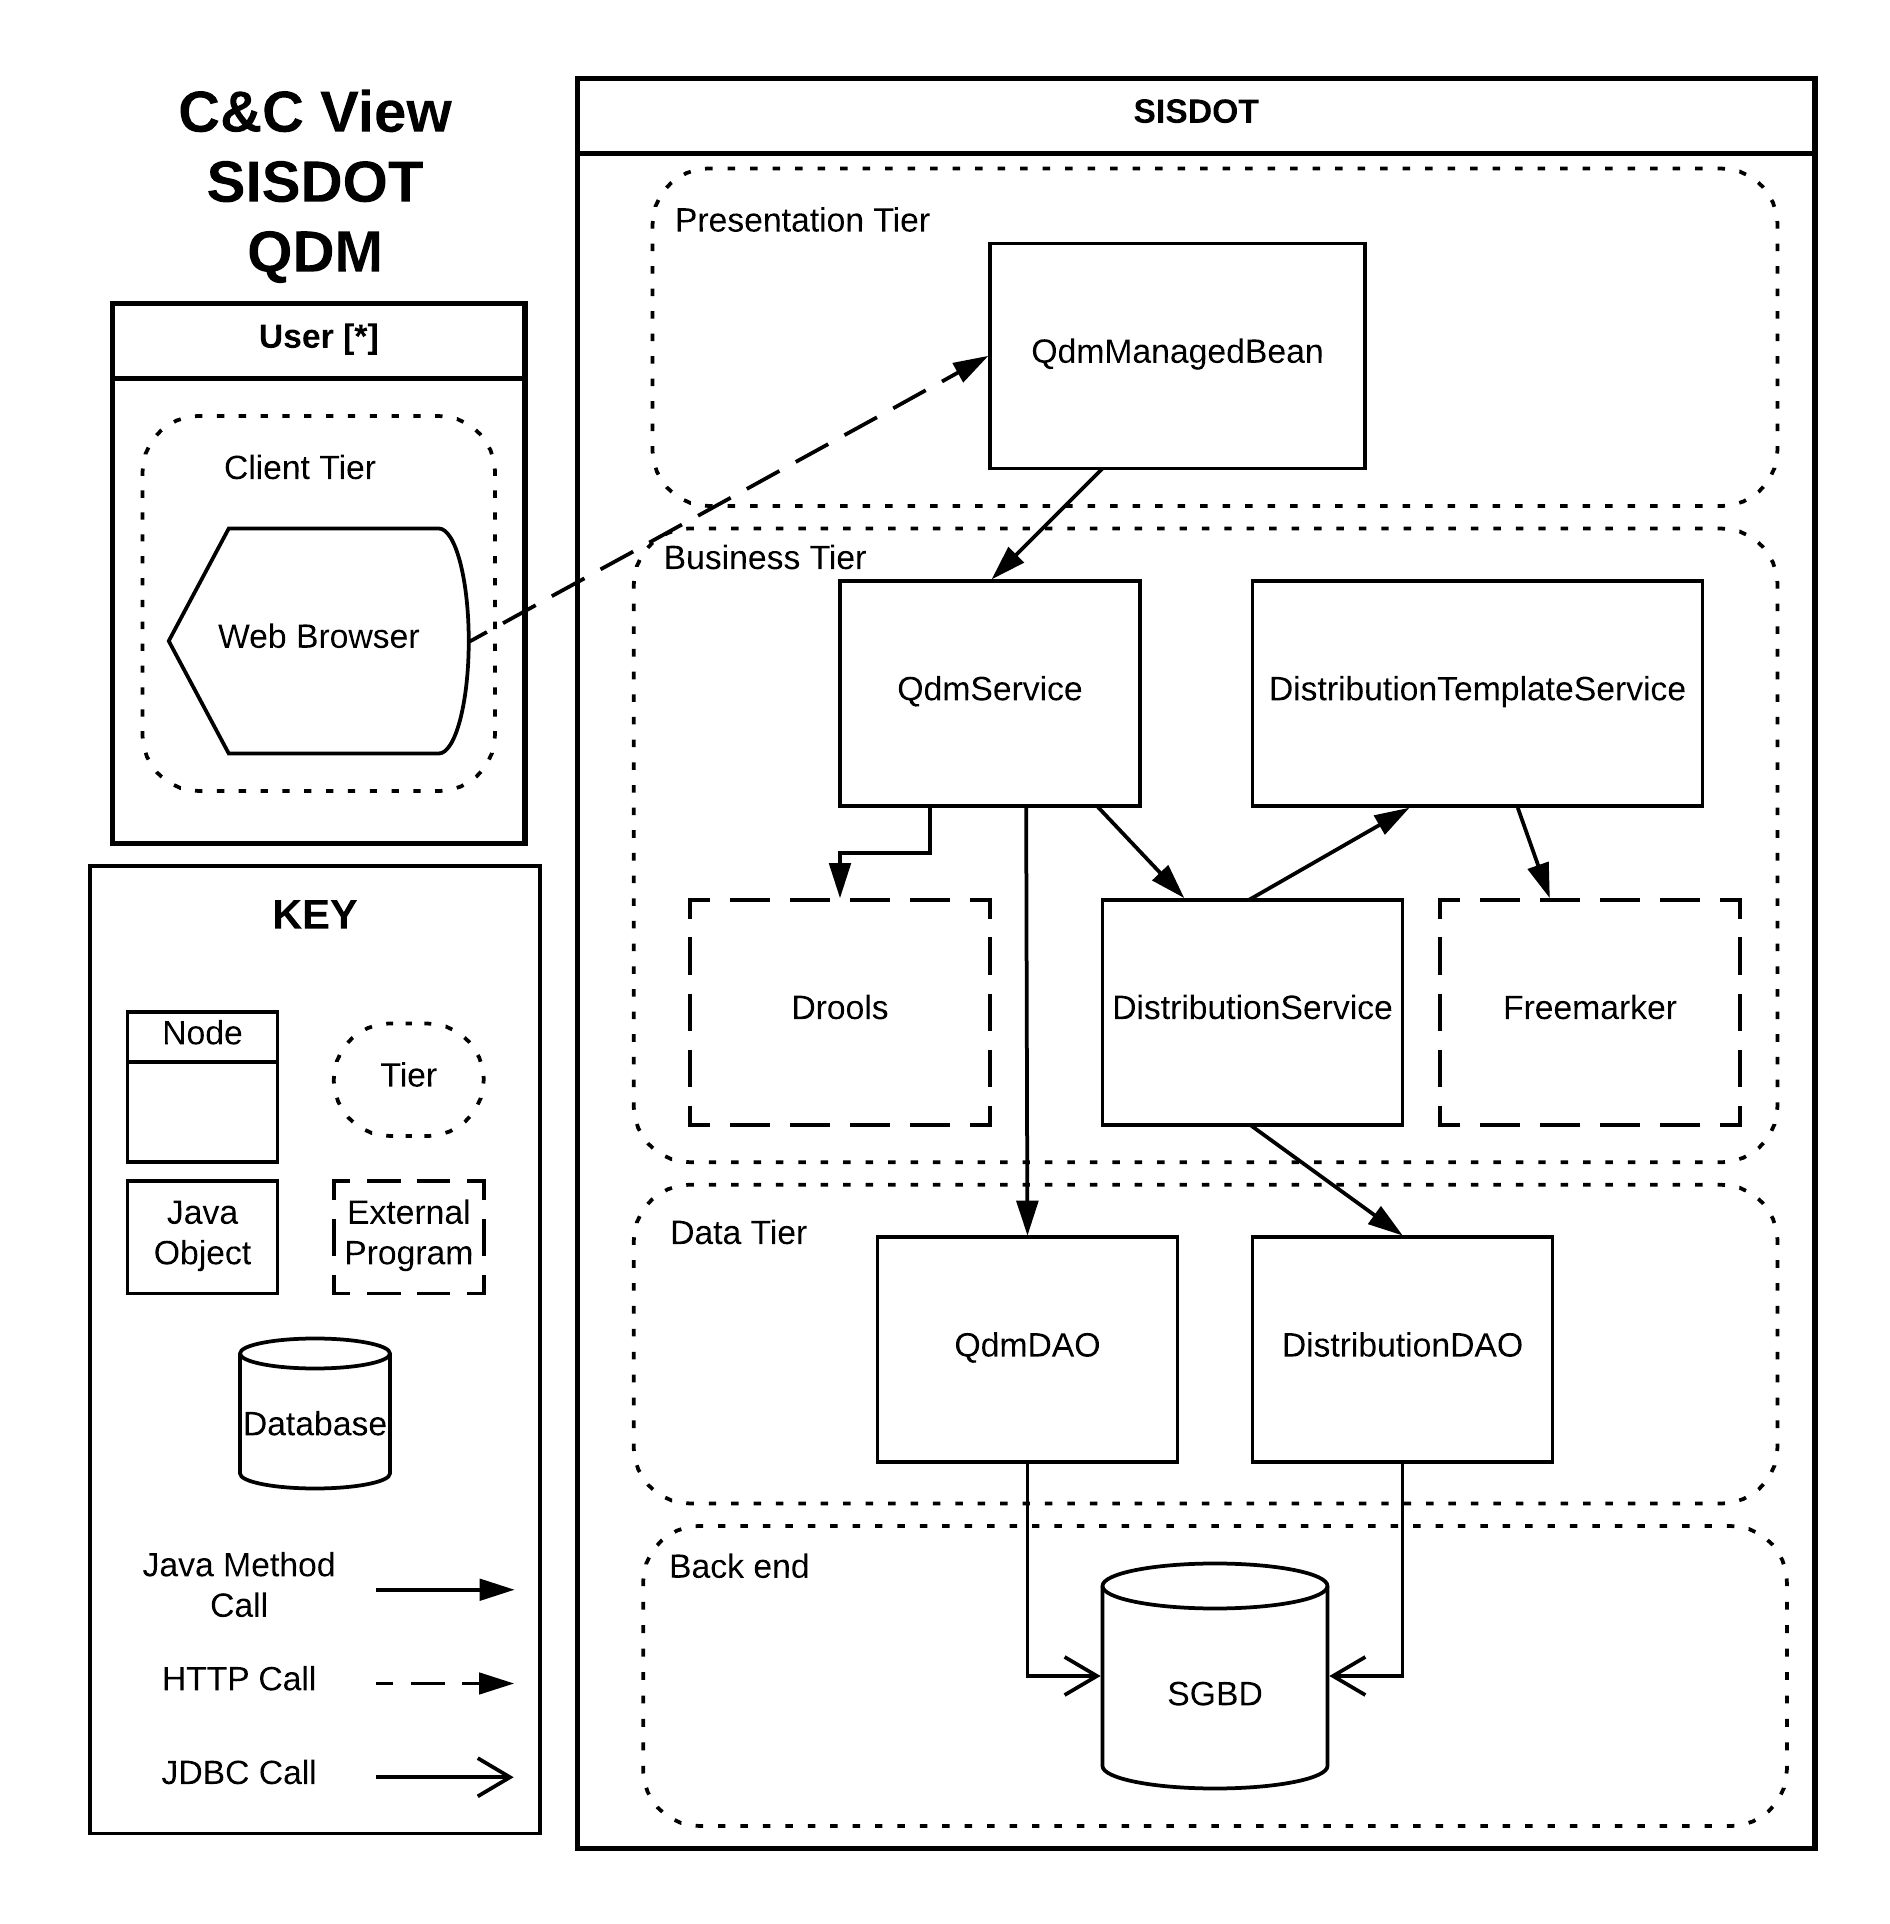
\includegraphics[scale=0.55]{img/runtimeView_qdm.png}
\caption{Runtime view of the architecture} 
\label{fig:fig:runtime_qdm}
\end{figure}
%\end{figure*}

\begin{lstlisting}[frame=single, float=*, language=DRL, caption=Example of a \emph{low-level Drools rule}, label={code:drl}]
rule "HLR 1"   	
when
  $qc: QuadroDeCargosVO(operational == OPERATIONAL)	
  $roles: List( size > 0 ) from accumulate ( 
     $dep: DepartmentVO(depId not in (14086, 1130)) from $qc.deps and
     $role: RoleVO(function == "ROLE", roleId in (2, 12, 15, 21)) from $dep.roles and  		
     QualificationVO(code in ("782", "756")) from $role.qualifications;				
    collectList( $role ))	 		
then		 
	for(int i=0; i < $roles.size(); i++){       	
		RoleVO c = (RoleVO) $roles.get(i);
		helper.add(1051000007, c.getFractionId(), c.getRoleId());   
end
\end{lstlisting}

\emph{Considering the user interaction}, a previously authenticated specialist on the 
distribution of equipment throughout the Brazilian Army, using her web browser, 
requests the web page that allows the generation of QDMs (one of the main products of SISDOT). 
After selecting the \emph{generic organizational unity} for which a QDM would be 
generated, the system sends a request to the server. The client tier is responsible for these actions. 
The request is then received by a component of the presentation tier, more specifically by a \emph{managed bean} that works 
as a \emph{front controller} (in this case, a JSF controller). 

This controller validates  
the request data, before sending a new request to the business tier. In the business tier, the service 
that implements the business rules related to the QDM domain object is invoked to start the QDM generation process, 
which includes actions to (a) transform \callers into the \emph{low-level rules} specified
using the Drools Rule Language (DRL), 
(b) execute these rules to instantiate a business object that represents a QDM, and (c)
save this object in the persistence layer (a relational database). 

This process for generating a QDM starts by retrieving a list of 
previously registered \callers. An \shc, regardless of its type (either based on the 
full structure of the organization or based on its components), 
is related to one or more \emph{military materials / equipment} (MEMs) 
and defines the respective amount that should be assigned to a military 
unit (which ranges from an organization, a center, a department, a brigade, or even 
a military function or qualification of a soldier). 

A high-level rule has one or more distribution rules. Each rule has a type, 
a value, and an associated description. For example, a rule for a 
department type has the value of the department identifier and the description of 
the department name. For a better use of the database, avoiding the definition 
of numerous columns that would inevitably be null for several rule types, we decided 
to persist the distribution rules of an \shc using JSON (JavaScript Object Notation), which is 
converted back to an object when it is retrieved. The set of these rules defines 
exactly who should receive the MEMs specified by the \shc.

% Um dos fatores que motivou o uso de um rule engine foi a similaridade entre chamadores e as regras 'se-então' características destes mecanismos. Um chamador possui um conjunto de condições que se encaixam na parte condicional de uma regra ('se') e possui uma série de ações ('então') que, no caso, são os MEMs que devem ser distribuídos em consequência da validade das condições. A estrutura básica de uma DRL pode ser vista na Listing \ref{code:drlStructure}.

One of the factors that motivated the use of a rule based engine was 
the similarity between \callers and the ``if-then'' rules of these mechanisms.  
%whose essential structure is shown in Listing~\ref{code:drlStructure}.
An \shc has a set of conditions that fits the conditional part of a rule (``if'') 
and has a set of actions (``then'') that, in this case, trigger the distribution 
of MEMs throughout the expected military unities.

%\newpage

%\begin{lstlisting}[frame=single, caption={Structure of a rule specified in Drools}, label={code:drlStructure}]
%rule "name"
%    attributes
%    when
%        LHS
%    then
%        RHS
%end
%\end{lstlisting}


The list of retrieved \callers contains only Java objects. 
In order to be able to use the rule engine in a transparent way for the end users 
(and also for developers in future maintenance scenarios), we decided to use a 
meta-programming approach, translating these objects into a set of rules (a program in 
logic programming) that might be used by a rule-based engine. As mentioned before,  
we decided to use the \emph{Drools rule-based engine} in the context of 
SISDOT (Figure \ref{fig:fig:runtime_qdm}), mostly because of its integration capabilities 
with both JEE systems and the Wildfly application server. Accordingly,  
the \callers are translated into DRL rules (Listing~\ref{code:drl} presents an
example of a \emph{low-level Drools rule}). To this end, we use a template engine (FreeMaker) 
to implement this particular transformation (Figure \ref{fig:fig:runtime_qdm}), using a template 
that contains the required \emph{markups} for transforming \shc into \emph{low-level} Drools 
rules. That is, for each \shc, the template engine populates the template, 
resulting in a DRL rule consistent with the converted \shc.
A code snippet of the template used for DRL generation can be seen in Appendix A. 

The RHS of the Drool rule of Listing~\ref{code:drl}
iterates over all selected military roles (that satisfy
the constraints of the LHS). We use a helper class to
assign the equipment id (in this case a \emph{rifle} whose id is
1051000007) to the individual roles. Besides providing
means to populate a QDM, this helper class also checks
some constraints related to the QDM domain model. 
%\begin{figure}[!ht] \centering
%	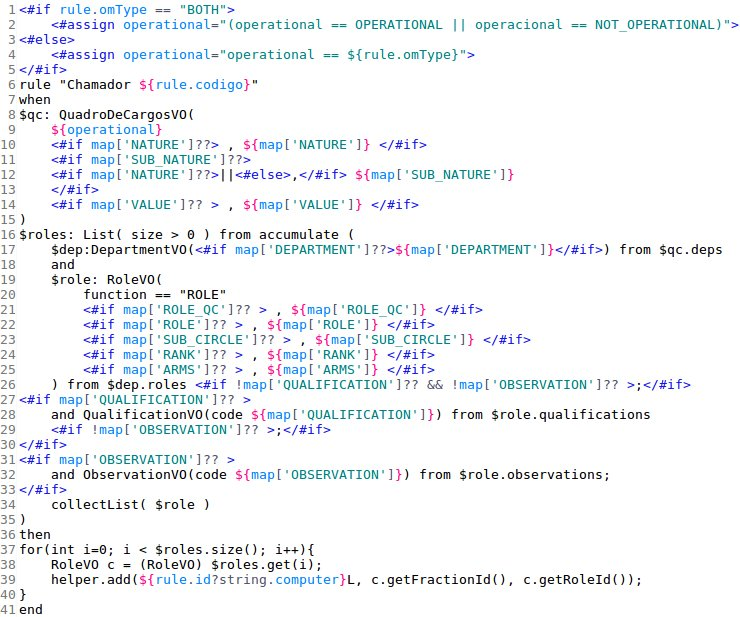
\includegraphics[width=.48\textwidth]{img/artigo_template.jpg}
%	\caption{\it Freemarker template for generating DRL} 
%	\label{fig:template}
%\end{figure}


A QDM is generated for a generic organizational unity (hereafter QC, from \emph{Quadro de Cargos} in Portuguese), 
selected by the user on the client tier. 
Therefore, the user-specified QC must be retrieved from the Brazilian Army's enterprise database  
through a specific Data Access Object (DAO) in the data tier~\cite{alur2003}.
From the list of DRL rules, created based on existing \callers, the rule engine is instantiated and these rules are compiled, 
so that they can be triggered by Drools. The QC domain object is then inserted into the working memory as a fact,  an 
information that is always considered true. The rules are only executed when their conditions are satisfied, 
based on the specified QC organizational structure. When a rule is valid, that is, it has been activated 
and the \emph{Left Hand Side} (LHS) conditions are valid, 
the QDM is populated with the MEMs specified in the \emph{Right Hand Side} (RHS) of the rules. Therefore, we generate a 
complete QDM object after verifying all valid rules (previously registered in the database) for 
the selected QC. 

After generating a QDM domain object, it is saved on the database and we let the domain expert know 
of the success of the operation using a simple user interface message. 
The domain expert can then perform the necessary operations on the generated QDM, including a workflow 
involving  its edition, homologation, and validation.  

\subsection{A Domain Specific Language for testing QDM Generation}

As explained before, to generate a QDM, a set of \callers must be previously 
declared. This is a time-consuming task, particularly when using the interface of 
the system. In order to facilitate the definition of the \callers used in the automated test scripts, we 
decided to implement \hlrdsl---a DSL (Domain Specific Language) that enables us to specify \callers in a 
clear, objective, and declarative way (and most important, without using the interface of the SISDOT system). 

We implemented \hlrdsl  using Xtext, which generates plugins that allow
code editing in both Eclipse and IntelliJ, plus an editor that can be
embedded in a web application. This way, a developer writing test scripts might
use \hlrdsl to take advantages of the functionality provided by these plugins.
To implement a DSL using Xtext, it is first necessary to declare a grammar expressed
using a syntax similar to ANTLR~\cite{parr2013}. Listing~\ref{code:gramatica} presents
the grammar of our DSL. From this grammar,the Xtext tool suite generates a lexer, a parser, a
set of classes representing the AST (Abstract Syntax Tree), and an editor with several features
typically available in IDEs.
% Although Xtext provides an interesting implementation for all
% these concerns, a language designer is also able to customize several of the Xtext
% outcomes~\cite{bettini2016}.

%\begin{figure}[!ht] \centering
%	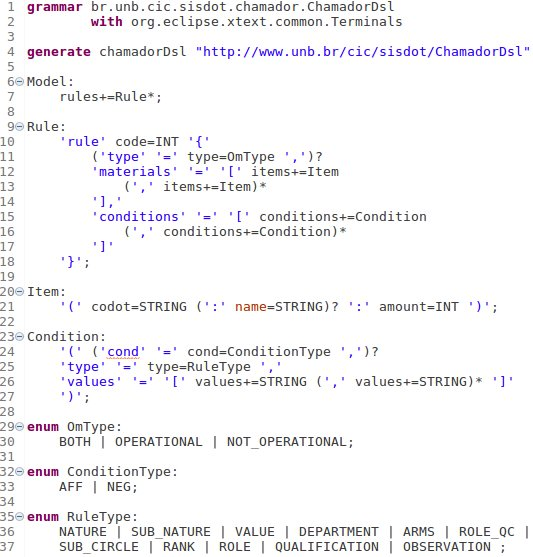
\includegraphics[width=.47\textwidth]{img/artigo_gramatica.jpg}
%	\caption{\it Xtext grammar defining the DSL structure} 
%	\label{fig:gramatica}
%\end{figure}
\begin{lstlisting}[frame=single, language=Xtext, caption={\it Xtext grammar defining the DSL structure}, label={code:gramatica}]
grammar br.unb.cic.sisdot.chamador.HLRDsl 
with org.eclipse.xtext.common.Terminals
generate hlrdsl "http://www.unb.br/sisdot/hlrdsl"

Model:
rules += Rule*;

Rule:
 'rule' code = INT '{'
  ('type' '=' type=OmType ',')?
   'materials' '=' '['items+=Item (',' items+=Item)*'],'
   'cnds' '=' '['cnds+=Condition (',' cnds+=Condition)*']'
'}';

Item: '(' codot=STRING (':' name=STRING)? ':' amount=INT ')';

Condition:
 '(' ('cond' '=' cond=ConditionType ',')?
 'type' '=' type = RuleType ','
 'values' '=' '[' values+=STRING (',' values+=STRING)* ']'
 ')';

enum OmType: BOTH | OPERATIONAL | NOT_OPERATIONAL;
enum ConditionType: AFF | NEG;
enum RuleType: NATURE | SUB_NATURE | VALUE | DEPARTMENT | ARMS | ROLE_QC | SUB_CIRCLE | RANK | ROLE | QUALIFICATION | OBSERVATION ;
\end{lstlisting}

Listing \ref{code:dslExample} presents a simple example of a \shc declaration using our DSL. 
The goal of this rule is to distribute 
the materials (defined in the list of materials construct) for \emph{operational} OMs (see the 
type construct) and militaries \emph{not working in the specified list of 
departments} with a set of qualifications and roles. While the definition of this rule 
using our DSL requires 12 lines of code, the corresponding definition of the same rule 
using a Java test case requires more than 50 lines of imperative code.

% {\color{red}A DRL gerada para o chamador da Listing \ref{code:dslExample} pode ser vista na} Listing \ref{code:drl}.  {\color{red} Na parte RHS da regra, há uma iteração sobre todos os cargos selecionados. Para cada cargo uma classe que auxilia o preenchimento do QDM é chamada para que os itens declarados no chamador, passado como parâmetro, sejam disponibilizados para o cargo. Essa classe auxiliar recupera o chamador passado como parâmetro a partir da lista de chamadores declarados na DSL, que foram convertidos em objetos Java. Além de auxiliar no preenchimento do QDM, esta classe popula alguns objetos que facilitam a verificação da consistência do QDM, por exemplo.}
% Converting the \shc of Listing~\ref{code:dslExample}
% leads to the \emph{low-level Drool rule} of Listing~\ref{code:drl}.

Our typical test approach consists first in the specification of the required \callers in a \hlrdsl
file. Next, the \emph{behavior under test} is detailed as features using
the Cucumber~\cite{wynne2017cucumber} framework (we present an 
example of a feature in Listing \ref{code:cucumber}). After that, the developer details 
the implementation steps of the features by (a) specifying which \callers
(previously declared using our DSL) should be considered 
in the test execution, (b) specifying which QC the QDM should be generated,
and (c) specifying the expected results in terms of the properties of the expected QDM. 
To this typical scenario, we use a testing  infrastructure that supports several facilities,
that aims to increase productivity, such as: database connectivity,
auxiliary methods for executing queries in the database, and predeclared rules in the rule engine.

\begin{small}
\begin{lstlisting}[frame=single, language=DSL, caption={\it Example of a \shc declaration using our DSL}, label={code:dslExample}]
rule 1 { 
 type = OPERATIONAL, 
 materials = [ 
   ("1051000007" : "Rifle" : 1), 
   ("1020100011" : "Rifle Carrying Case" : 2)
 ], 
 cnds = [ 
  (cond=NEG, type=DEPARTMENT, values=[14086 , 1130]),
  (type=QUALIFICATION, values=[782, 756]), 
  (type=ROLE, values=[2, 12, 15, 21])
 ]
}
\end{lstlisting}
\end{small}


That is, \hlrdsl simplifies the process of specifying \callers and its primary goal was to 
assist in test activities. However, after presenting to domain experts some examples of \callers specified using 
our DSL, we realized that \hlrdsl might also be useful  
to simulate the specification of rules, allowing a better understanding of the effect of each 
\shc for building QDMs.


%\begin{figure}[!ht] \centering
%	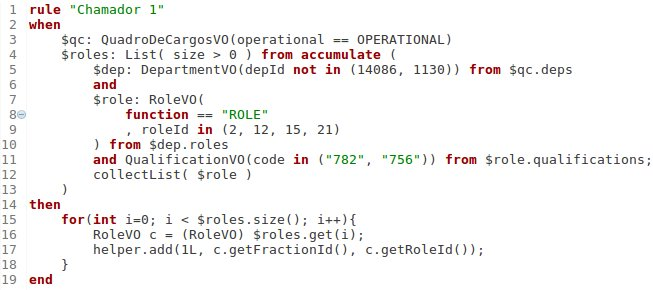
\includegraphics[width=.48\textwidth]{img/artigo_drl.jpg}
%	\caption{\it DRL generated} 
%	\label{fig:drl}
%\end{figure}


Our second approach for testing automatically generates test cases 
from our DSL and from a random sample of simple combinations that
characterize artificial organizational unities. This \emph{property
based approach} involves a custom Maven plugin that currently generates simple test cases, 
freeing the tester to create only complex tests related to the QDM generation. 
These test cases are generated from a combination of conditions, for example:
one test case only for operational OMs 
and another for non-operational OMs; a test case for the different kinds of OMs (artillery, infantry,
cavalry, aviation and helicopters, general services, and so on), combining with the operational type, 
such as: operational infantry OMs and non-operational infantry OMs. These combinations are generated for simple 
cases so that they are easy to verify without the need to manually implement
Java test scripts for generating QDMs. 

%\begin{figure}[!ht] \centering
%  \includegraphics[width=.32\textwidth]
%  {img/plugin.jpg}
%  \caption{\it Maven plugin for test generation}
%  \label{fig:pluginExample}
%\end{figure}
\begin{lstlisting}[frame=single, language=Plugin, caption={\it Maven plugin for test generation}, label={code:plugin}]
<plugin>
  <groupId>xxx</groupId>
  <artifactId>xxx</artifactId>
  <executions>
    <execution>
      <id>execute</id>			
      <configuration>
        <seed>10</seed>				
        <qcs>702311,762314,575311</qcs>				
      </configuration>
      <goals>
        <goal>generate</goal>
      </goals>
    </execution>
  </executions>
</plugin>	
\end{lstlisting}

In this second approach, for each of the possible combinations, we generate a \shc that meets the conditions 
and a cucumber feature that exercises the \shc and compares the expected results declared in the feature. 
Each \shc is considered during the generation of the QDM to the QCs specified in the 
maven plugin (as shown in Listing~\ref{code:plugin}).
That is, to use this architecture characteristic (here we consider testability as an 
architecture concern), we ``feed'' the maven plugin with a list of QC codes for which the QDMs should be generated, 
besides other optional information, which have default values, such as: database connection string,
seed to be used in the random selection of values within a combination (e.g., considering 20 different
kinds of organizational units, randomly take 5 for generating the set of combinations), and the output directory 
where the code should be exported. 

%\begin{figure}[!ht] \centering
%  \includegraphics[width=.45\textwidth]
%  {img/artigo_cucumber.jpg}
%  \caption{\it Cucumber feature}
%  \label{fig:cucumber}
%\end{figure}
\begin{lstlisting}[frame=single, language=Cucumber, caption={\it Cucumber feature}, label={code:cucumber}]
Feature: QDM 757311
	As a user
	I want to generate a QDM from HLRs

	Scenario: Test 1
		Given QC with code 757311
		And HRL: 1, 2
		When I generate a QDM
		And the results are consistent
		Then positions must be populated
		| idDep    | idPos   | codot      | amount |
		| 6765748  | 10403   | 1051000025 | 1      |
		| 6765748  | 10403   | 1020100017 | 1      |
		| 6765748  | 10403   | 1020100013 | 1      |
		| 6765748  | 10403   | 1051000006 | 1      |
		| 6765748  | 21328   | 1051000025 | 1      |
		| 6765750  | 10122   | 1051000025 | 1      |    
		| 6765793  | 13276   | 1051000025 | 6      |
		| 6765796  | 24655   | 1051000025 | 1      |
		| 6765796  | 24429   | 1051000025 | 2      |
		| 6765798  | 24429   | 1051000025 | 3      |
		| 6765798  | 11433   | 1051000025 | 9      |   
		And the final result must be:
		| codot      | amount |
		| 1020100013 | 74     |
		| 1020100017 | 74     |
		| 1051000006 | 74     |
		| 1051000025 | 74     |

	Scenario: Test 2
		Given QC with code 757311
		And HRL: 1, 2, 3
		When I generate a QDM
		And the results are inconsistent    
\end{lstlisting}



After running the plugin, with the generated code, the tests are executed in a similar way to the test 
definitions detailed before. The tests run along with the other unit tests declared, 
whether DSL-based or not.
 
\section{Case Study}
\label{sec:case_study} 


For the validation of the proposed architecture we conducted a case study, which consists of the evaluation of the main 
architectural decisions of SISDOT, which relate to the generation of QDMs. The case study aims to answer the 
following research questions:

\begin{itemize}

% \item \textbf{RQ.1}: O uso da DSL na execução de testes reduz o esforço do profissional de testes durante a implementação dos casos de testes?
\item \textbf{RQ.1}: Does our proposed approach, based on meta-programming, generate correct QDMs?

\item \textbf{RQ.2}: Does the use of a DSL reduce the effort necessary to implement the test cases that target QDM generation? 

\item \textbf{RQ.3}: Does our proposed approach, based on meta-programming, generate QDMs within a satisfactory time-frame?

\end{itemize}

% A RQ.1 está relacionada à produtividade do testador e demonstra quanto código a menos o desenvolvedor deve implementar ao utilizar a DSL criada, em comparação com a declaração do mesmo chamador utilizando a linguagem Java. Apesar de não haver formalmente um requisito funcional especificando qual seria um tempo aceitável para a geração de um QDM, foi determinado que um tempo maior que 5 segundos, ao utilizar 1000 chamadores, é inaceitável. Assim, a RQ.2 serve para garantir que os QDMs sejam gerados em tempo satisfatório.

\textbf{RQ.1} deals with the most important concern: correctness regarding the QDM generation. It is intended 
to demonstrate that the solution not only automatically generates the rules, eliminating the work that the developer 
would have to implement the solution in Java, but also that the proposed approach leads to the expected QDMs when considering 
a well defined set of \callers.
\textbf{RQ.2} is related to the productivity of the tester and demonstrates how much code the 
developer have to write when using our DSL, compared to the effort to specify \callers using the Java language in 
unit test cases. Although there is no formal functional requirement specifying the  acceptable time for generating a QDM, 
it has been determined that a time greater than 5 seconds, when using 1000 \callers, would be unacceptable. 
Thus, \textbf{RQ.3} serves to ensure that the QDMs are generated in a satisfactory time.

% Com a RQ.3 pretende-se demonstrar que a solução gera as regras automaticamente, eliminando o trabalho que o desenvolvedor teria para implementar a solução em Java. Com poucas linhas de código, relacionadas à definição do template e sua execução, a solução gera um arquivo de regras com determinado número de linhas de código Drools. A resposta dessa questão está relacionada aos resultados dos testes manuais e automáticos.


\subsection{Data Collection and Analysis}

% A coleta dos dados foi realizada utilizando as seguintes métricas: linhas de código (LOC) e tempo de execução. A escolha dessas duas métricas está relacionada ao tamanho do código, que pode indicar uma maior produtividade; e à satisfação do requisito funcional que determina o tempo máximo de execução para a geração de QDM. 
We answer our first question qualitatively. Although this might look like disappointing (under the 
perspective of empirical methods), we have strong evidences collected from the domain experts 
that our approach has produced correct QDMs. We believe that this correctness is due to several 
factors, including the involvement of the domain experts that helped us to full understand 
the requirements and the expertise of our development team. Nevertheless, the decision of 
not writing the low-level rules at the source code level, but instead using a program 
generation approach that has reduced significantly the effort needed to \emph{hand write} 
those rules, has also contributed to achieve this confidence about correctness. 

In a meeting 
with the domain experts, one of the specialists said: ``I got surprised with the 
correctness of the solution. In the previous version of the system, we had to have several 
interactions until we got confident about the correct operation of the \callers''. The first 
time that we generate QDMs, the process was validated. It is important to note that ``not all 
are flowers'', and we broke the initial implementation after the introduction of a new, 
at first not so related feature that, in the end, cut across several classes of 
the system. We fixed the related issues recently.  

To answer the other two research questions, we collected the following metrics: lines of code (LOC) and execution time. The choice of these 
two metrics is related to the size of the code, which may indicate higher productivity; and to the fulfillment of the 
functional requirement that determines the maximum execution time for the generation of QDMs.

%A Tabela \ref{table:comparacao} apresenta a comparação dos resultados obtidos utilizando DSL e Java. 

\begin{table}[htb!]
\centering
\caption{Comparing the number of lines of code need to specify test cases using our DSL and Java}
\label{table:comparacao}
\begin{center}
\begin{tabular}{ccc}
\hline
\textbf{\shc Code} & \textbf{Lines of Code (DSL)} & \textbf{Lines of Code (Java)}     \\ \hline 
1        & 10  & 26   \\ \hline
2        & 10  & 25   \\ \hline
3        & 10  & 32   \\ \hline
4        & 11  & 52   \\ \hline
5        & 15  & 41   \\ \hline
6        & 9   & 16   \\ \hline
7        & 18  & 21   \\ \hline
8        & 12  & 25   \\ \hline
15       & 7   & 45   \\ \hline
58       & 7   & 58   \\ \hline
59       & 17  & 34   \\ \hline
\end{tabular}
\end{center}
\end{table}

% No cenário de testes considerado para o estudo de caso, o sistema SISDOT possuia  66 chamadores declarados em sua base de dados. Esses chamadores correspondem a chamadores reais utilizados pelo Exército Brasileiro (EB) para a realização de alguns testes na geração de QDMs. A conversão de cada chamador escrito na linguagem Java para o seu correspondente no formato da DSL foi realizada com o uso do Xtext. A Table \ref{table:comparacao} apresenta uma amostra dos dados coletados. A primeira coluna contém o código do chamador, a segunda coluna contém a quantidade de linhas de código para representar o chamador na DSL e a terceira coluna contém a quantidade de linhas para representar o mesmo chamador na linguagem Java.

We use as a benchmark 66 \callers declared in its database. These \callers correspond to real rules used by 
the Brazilian Army to perform some tests related to the generation of QDMs. We converted  
each \shc written using JUnit to their correspondent one specified using our DSL. 
Table \ref{table:comparacao} presents a sample of the collected data. The first column contains 
the \shc code, the second column contains the number of lines of code to represent the \shc using our DSL, and the third 
column contains the number of lines to represent the same rule in the Java language.

% Para a coleta da métrica de tempo de execução foi utilizado um computador com processador Intel(R) Core(TM) i7-4790, com 16GB de memória RAM, com o sistema operacional Ubuntu 16.04.4 LTS, 64 bits, com kernel 4.15.0-24-generic. Foram usados 16 QCs, escolhidos de forma a representar os variados tipos de OM, naturezas e subnaturezas. Para cada QC foram gerados QDMs usando as seguintes quantidades de chamadores: 20, 40, 50, 60, 100, 200, 400, 700, 1000, 1500, 2000, 3000, 5000. Como só haviam 66 chamadores reais já declarados, os conjuntos com quantidade maior contém chamadores repetidos. A seleção dos chamadores foi realizada de maneira randômica, mas com o mesmo seed, para que os mesmos conjuntos fossem utilizados nas gerações dos QDMs de diferentes QCs. A Table \ref{table:tempo} apresenta uma amostra dos resultados obtidos com a execução. A primeira coluna contém o código do QC, e da segunda coluna em diante contém o tempo, em milisegundos, para a geração dos QDMs usando a quantidade de chamadores indicada no header da respectiva coluna.

Regarding the runtime metrics, we collected the data using an Intel(R) Core{TM} i7-4790 processor, 
with 16GB of RAM, running Ubuntu 16.04.4 LTS 64-bit operating system, with 4.15.0-24-generic kernel. We used 16 QCs, 
chosen to represent the various OM types, natures, and subnatures. For each QC, we generated QDMs using 
random sets of \callers with size: 20, 40, 50, 60, 100, 200, 400, 700, 1000, 1500, 2000, 3000, 5000. 
Since there were only 66 real \callers already declared, larger quantities contain repeated callers (which in the end will duplicate 
the data within a given QDM). The selection of callers was performed at random, but with the same seed, so that the same sets were used in the 
generation of QDMs for different QCs. Table \ref{table:tempo} shows a sample of the results obtained with the execution. 
The first column contains the QC code, and the second column contains the time in milliseconds for the generation of 
the QDMs using the indicated amount of \callers on the respective column header.

\begin{table}[htb!]
\centering
\caption{Time (ms) for generation of QDMs}
\label{table:tempo}
\begin{center}
\begin{tabular}{|l|l|l|l|l|l|l|}
\hline
\textbf{QC}      & \textbf{60}  & \textbf{100} & \textbf{400}  & \textbf{700}  & \textbf{1000} & \textbf{2000} \\ \hline

206410  & 184 & 275 & 944  & 1829 & 2279 & 4707 \\ \hline
231303  & 197 & 282 & 975  & 1731 & 2541 & 4987 \\ \hline
500311  & 201 & 291 & 948  & 1804 & 2289 & 4950 \\ \hline
618322  & 175 & 264 & 922  & 1640 & 2412 & 4990 \\ \hline
727310  & 173 & 302 & 937  & 1652 & 2466 & 4992 \\ \hline
1450311 & 182 & 269 & 890  & 1649 & 2527 & 4785 \\ \hline
2203310 & 197 & 263 & 909  & 1619 & 2344 & 4976 \\ \hline
5406194 & 176 & 253 & 884  & 1598 & 2393 & 4610 \\ \hline
7020003 & 212 & 241 & 922  & 1610 & 2361 & 4470 \\ \hline
9131000 & 171 & 252 & 888  & 1609 & 2345 & 4471 \\ \hline
\end{tabular}
\end{center}
\end{table}

We exported the collected data to the CSV format, so that we could perform a data analysis using the R environment~\cite{crawley2013}. 
In the data analysis for \textbf{RQ.2}, which compares the number of lines of code between the two distinct approaches for 
representing \callers, we created two additional columns: \emph{difference}, which measures the difference in the number of 
lines of code necessary to specify \callers using Java and our DSL; and \emph{percent of reduction}, which indicates 
how much less code is necessary to specify a \shc using our DSL, when compared to the direct specification in Java code.

\begin{table}[htb!]
\centering
\caption{Analysis of DSL and Java comparison data}
\label{table:analiseComparacao}
\begin{center}
\begin{tabular}{|l|l|l|l|l|l|}
\hline
           & \textbf{Min.}  & \textbf{Median} & \textbf{Mean}  & \textbf{SD}    & \textbf{Max.}  \\ \hline
DSL        & 7.00  & 9.00   & 9.67  & 2.81  & 18.00 \\ \hline
Java       & 9.00  & 17.50  & 21.76 & 14.68 & 96.00 \\ \hline
Difference & 2.00  & 7.00   & 12.09 & 13.94 & 83.00 \\ \hline
\%         & 14.29 & 43.75  & 45.23 & 19.84 & 87.93 \\ \hline
\end{tabular}
\end{center}
\end{table}

% Na Table \ref{table:analiseComparacao} é possível observar algumas estatísticas descritivas dos dados coletados, contendo as seguintes colunas: valor mínimo, mediana, média, desvio padrão e valor máximo. Existe uma forte correlação entre as colunas Java e Difference, de 0.982. Essa correlação pode ser visualizada na Figure \ref{fig:correlacao}. É possível identificar que a medida que o tamanho do código Java cresce a diferença para a representação em DSL também aumenta. 

Table \ref{table:analiseComparacao} presents some descriptive statistics 
of the collected data, containing the following columns: minimum value, median, mean, standard deviation, and maximum value. 
There is a strong correlation (0.982) between the lines of code in Java and the \emph{difference} measurements. 
This correlation can be seen in Figure \ref{fig:correlacao}. It is possible to identify that as the size of the Java code grows, 
the difference for the representation in DSL also increases.

\begin{figure}[htb!] 
\centering
  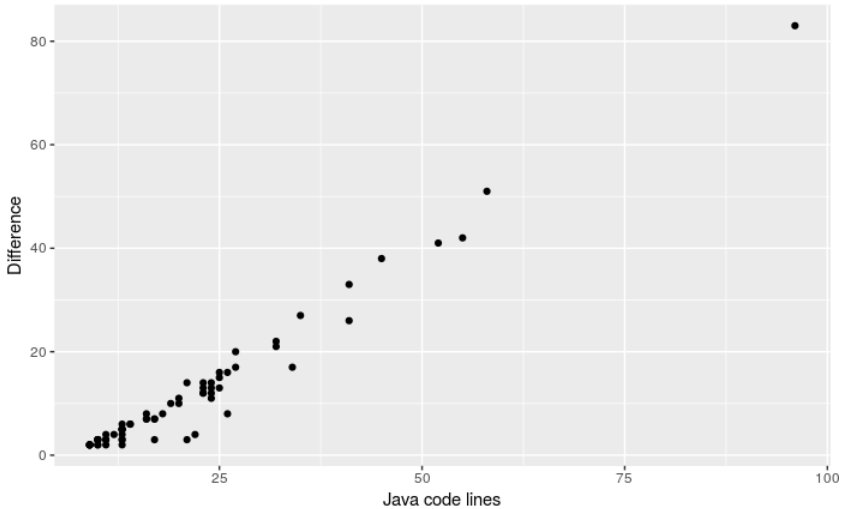
\includegraphics[width=.48\textwidth]
  {img/artigo_correlacao.jpg}
  \caption{\it Correlation between Java and Difference}
  \label{fig:correlacao}
\end{figure}

Figure \ref{fig:geracao} shows the time necessary to generate QDMs for 5 different QCs. For each of them, 
6 QMS were generated, with different amounts of \callers, 60, 100, 400, 700, 1000 and 2000.

\begin{figure}[!ht] \centering
  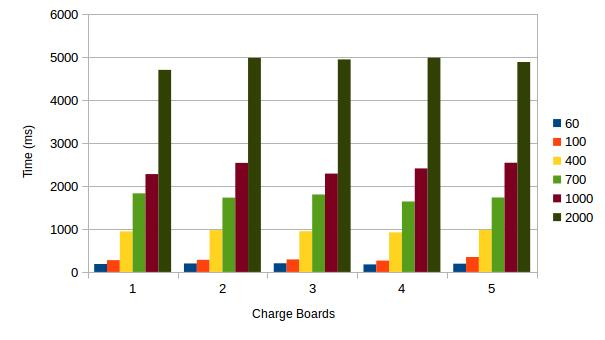
\includegraphics[width=.48\textwidth]
  {img/artigo_geracao.jpg}
  \caption{\it QDM Generation Time (ms)}
  \label{fig:geracao}
\end{figure}

\subsection{Discussion}

When analyzing the data related to RQ.2, it was possible to observe that the representation 
of a \shc using our DSL is on average 45\% smaller than the representation of the same rule in Java. 
This indicates a possible productivity gain for the developer when writing test cases, 
since her will have to write a smaller amount of code. In addition, using our DSL, we 
specify \callers using a declarative approach, which is close to the vocabulary of 
the problem domain. 
With respect to the third research question, the limit imposed by the functional requirement of 5 seconds was not exceeded,  
even when considering 2000 \callers, which is twice the number of \callers expected for the system 
in production.

\subsection{Threats to validity}

% Foram usados apenas 66 chamadores reais, que serviram de base para medir o tempo de geração de QDMs. Espera-se que o SISDOT tenha por volta de 1000 chamadores, quando o mesmo estiver em ambiente de produção. Apesar da pequena quantidade de chamadores utilizada, incluindo suas repetições quando necessário, é esperado que o sistema cumpra o requisito funcional, pois os testes com o dobro de chamadores esperados ainda estão dentro do tempo máximo aceitável de 5 segundos para geração de QDM.

We only consider 66 real \callers in our study, which served as a basis for measuring the generation time 
of QDMs. SISDOT is expected to have around 1000 \callers in the production environment. To mitigate the threat 
related to the small number of available \callers for testing, we consider their repetition when carrying out the 
performance test of the application. In this way, we expect that the system would present a behavior similar 
to the production environment (with respect to performance). The same situation occurs with the comparison 
of lines of code between the declarations of \callers in DSL and Java. As the number of callers is relatively small, 
it may not be possible to generalize the results we found.
 
\section{Final Remarks}
\label{sec:conclusao}

% O objetivo desse trabalho foi descrever as principais decisões arquiteturais e de design adotadas para implementar os mecanismos para derivar regras de negócio de alto nível em regras específicas para o motor de regras Drools e a definição de uma DSL que facilita a declaração de regras de negócio de alto nível. Além da apresentação do início do trabalho para geração automática de testes para complementar os testes definidos manualmente.

In this paper we detailed the main design and architectural decisions we use to 
implement the mechanisms necessary to support the distribution of materials 
through the Brazilian Army unities. These decisions included the use of 
a metaprogamming approach to derive high level business rules in rules specific to a rule 
based system (Drools) and the definition of a DSL that facilitates the declaration of \callers 
to build test scripts. 

% Foi realizado um estudo de caso para validar a arquitetura proposta a partir da avaliação do principal caso de uso do SISDOT, relacionado à geração de QDMs. A partir dos resultados obtidos com o estudo de caso foi possível observar uma diminuição considerável, de 45\% em média, da quantidade de linhas de código necessárias para a declaração de um chamador usando a DSL criada em comparação com a representação do mesmo chamador em Java, indicando um possível ganho de produtividade para o testador. Outro resultado do estudo de caso demonstrou a aderência do sistema ao requisito funcional declarado, de limitar o tempo de geração de um QDM em 5 segundos. Esse limite não foi ultrapassado nem quando foi utilizado o dobro da quantidade de chamadores esperados para o sistema em produção.

We carried out an empirical study to validate the proposed architecture, based on the evaluation of one of the 
main scenarios of our logistic system (SISDOT), related to the generation of QDMs. From the results obtained, 
it was possible to observe a reduction in the average number of lines of code required for the declaration 
of a \callers using our DSL, in comparison with the representation of the same \shc in Java. 
Another result of the case study shows that our approach fulfills a non functional requirement that constraints 
the expected time to generate QDMs. This limit was not exceeded even when using twice the number of \callers 
expected for the system in production environment.

Although the architecture discussed here considers the specific needs of the Brazilian Army, 
we believe that logistic systems from other institutions might benefit from our technical 
decisions as well.

%% % Para refinar os resultados obtidos com a arquitetura proposta foram definidos os os seguintes trabalhos futuros:

%% To refine the results obtained with the proposed architecture, the following future works were defined:

%% \begin{itemize}
%% % \item Refactoring dos serviços de QDM para otimizar a sua geração;
%% \item Refactoring QDM services to optimize your generation;
%% % \item Finalizar a geração de testes automáticos de forma a responder à RQ.3;
%% \item Finish the generation of automatic tests in order to respond the RQ.3;
%% % \item Coletar e analisar as métricas novamente quando houver uma quantidade expressiva de chamadores, os quais continuam em constante criação pelo Exército Brasileiro, com o intuito de testar a arquitetura proposta.
%% \item Collect and analyze the metrics again when there is an expressive amount of callers, which are constantly being created by the Brazilian Army, in order to test the proposed architecture.
%% \end{itemize}


% \section{Acknowledgments}
% \label{sec:Acknowledgments}

% The authors would like to thank the Brazilian Army for their support to this work and to allow our University to conduct this research in the context of a real software modernization effort (FUB / CIC 6138/2016).

\bibliographystyle{ACM-Reference-Format}
\bibliography{bibliography}

\end{document}
